\documentclass[12pt]{article}

\usepackage{listings}
\usepackage{graphicx}
\usepackage{float}
\usepackage{hyperref}

\usepackage{amssymb} 
\usepackage{amsmath}
\usepackage{amsthm}
\usepackage{sansmath}
\usepackage{epsfig}

\usepackage[T1]{fontenc}
\usepackage{lmodern}
\renewcommand*\familydefault{\sfdefault}

\usepackage[margin=2cm]{geometry}

\usepackage[parfill]{parskip}
\linespread{1.2} 

\usepackage{xcolor}

\lstdefinestyle{code}{  
    commentstyle=\color{gray},
    keywordstyle=\color{blue},
    numberstyle=\tiny\color{gray},
    stringstyle=\color{teal},
    ndkeywordstyle=\color{purple},
    basicstyle=\ttfamily\footnotesize,
    breakatwhitespace=false,         
    breaklines=true,                 
    captionpos=t,                    
    keepspaces=true,                 
    numbers=left,                    
    numbersep=8pt,                  
    showspaces=false,                
    showstringspaces=false,
    showtabs=false,                  
    tabsize=4,
    frame=single,
    breaklines=true
}

\lstset{style=code}

\newcounter{question}
\setcounter{question}{0}
\newcounter{subquest}

\newcommand{\question}[1]{
    \stepcounter{question} 
    \vspace{1em}
    \textbf{\Large\thequestion \ - #1}
    \vspace{.5em} 
    \setcounter{subquest}{0}\ \\}

\newcommand{\subquestion}{
    \stepcounter{subquest} 
    \vspace{.5em}
    \textbf{\large Question \thequestion.\thesubquest}
    \vspace{.25em}\ \\}

\newcommand{\solution}
    {\par\vspace{0.5em}\noindent\emph{Solution.}\ }
    {\par\vspace{1em}}

\usepackage{fancyhdr}
\setlength{\headheight}{15pt}
\pagestyle{fancy} 
\lhead{Math 5334: \emph{Numerical Analysis}}
\rhead{Serena Su}
\cfoot{}
\rfoot{\thepage}

\begin{document}

\begin{center}
\textbf{\huge Assignment 2}

{\large\emph{Due Date: September 22, 2025}}
\vspace{1em}
\end{center}
\hrule

\question{Lagrange Interpolation and Error Analysis}
Let $f \in C^{n+1}[a,\,b]$, and let $P_n$ be its Lagrange interpolating polynomial at the distinct nodes $x_0, x_1, \dots, x_n \in [a,\,b]$. The interpolation error is: 
\[R_n(x) = f(x) - P_n(x) = \frac{f^{(n+1)}(\xi)}{(n+1)!} \prod_{i=0}^{n}(x - x_i),\quad \xi \in (a,\,b)\]
Suppose $f(x) = e^x$ on the interval $[0,\,1]$, for equally spaced nodes $x_i = \frac{i}{n}$.

\subquestion
Derive an explicit bound for the maximum error $\max_{x \in [0,1]} |R_n(x)|$.


\begin{proof}
    To bound $|R_n(x)|$, we start with the error formula:
    \[|R_n(x)| = \left|\frac{f^{(n+1)}(\xi)}{(n+1)!} \prod_{i=0}^{n}(x - x_i)\right|, \quad \xi \in (0,1)\]
    
    Note $\frac{1}{(n-1)!}$ is a constant. We can bound $R_n(x)$ by bounding $f^{(n+1)}(\xi)$ and $\left|\prod_{i=0}^{n}(x - x_i)\right|$ separately.
    
    Now notice that $f^{(n+1)}(x) = f(x) = e^x$ for all $n$. Since $e^x$ is strictly increasing on $[0,1]$, we have that \[f^{(n+1)}(\xi) = \max_{x \in [0,1]} |f^{(n+1)}(x)| = f(1) = e \label{f}\tag{1}\]

    Next, we need to bound $\left|\prod_{i=0}^{n}(x - x_i)\right|$. Let $\omega_{n}(x) = \prod_{i=0}^{n}(x - x_i)$. Note that $\omega_{n}(x)$ is a polynomial of degree $n+1$. Since $\omega_{n}(x)$ is continuous on the compact interval $[0,1]$, it attains its maximum at some point in $[0,1]$. We may write that: 
    \[|\omega_{n}(x)| \leq W_n \label{h}\tag{2}\]
    Where $W_n = \max_{x \in [0,1]} |\omega_{n}(x)| = |\omega_{n}(x^*)|$ for some $x^* \in [0,1]$.

    Now, we can use \eqref{f} and \eqref{h} to bound $|R_n(x)|$ from above:
    \[|R_n(x)| \leq \frac{e}{(n+1)!} W_n\]
    Since $R_n(x)$ is continuous on the compact interval $[0,1]$, $\sup_{x\in[0,1]} R_n(x) = \max_{x\in[0,1]} R_n(x)$. \\ Since the supremum is the least upper bound, we have that:
    \[\max_{x \in [0,1]} |R_n(x)| \leq \frac{e}{(n+1)!} W_n\]
    Which gives us an explicit bound for the remainder.
\end{proof}

\subquestion
Show the asymptotic decay of this error as $n \to \infty$.

\begin{proof}
    From the previous part, we have that:
    \[\max_{x \in [0,1]} |R_n(x)| \leq \frac{e}{(n+1)!} W_n\]

    Let us first make a more crude estimate of $W_n$. Note that for any $x \in [0,1]$ and for each $i$, we have:
    \[|x - x_i| \leq 1\]
    Since there are $n+1$ terms in the product, we can write:
    \[|\omega_{n}(x)| = \left|\prod_{i=0}^{n}(x - x_i)\right| \leq 1^{n+1} = 1\]
    Therefore, we get the crude bound:
    \[W_n = \max_{x \in [0,1]} |\omega_{n}(x)| \leq 1\] 
    Plugging this into our error bound, we get:
    \[\max_{x \in [0,1]} |R_n(x)| \leq \frac{e}{(n+1)!}\]
    Taking a limit as $n \to \infty$, we have:
    \[\lim_{n \to \infty} \max_{x \in [0,1]} |R_n(x)| \leq \lim_{n \to \infty} \frac{e}{(n+1)!} = 0\]
    Therefore, we have shown that the error decays to $0$ as $n \to \infty$.
\end{proof}

\newpage
\question{Interpolation Programming Exercise}
Consider the fuction:
\[f(x) = \frac{1}{1+20x}, \quad x \in[-1,1]\]

\subquestion
Construct the interpolation polynomial $P_n(x)$ at equidistant nodes for $n=5$.

\solution The following methods were used to compute this polynomial:

\begin{lstlisting}[language=Python, caption=2.1 Python]
import numpy as np

def f(x):
    return 1 / (1 + 20 * x**2)

def lagrange_coefficients(nodes, function=f):
    x = nodes
    num_nodes = len(nodes)
    # Add zeroth divided differences
    dd_table = np.array([[function(xi) for xi in nodes]])

    # Calculate divided difference table
    for i in range(1, num_nodes):
        ith_dd = np.zeros(num_nodes)

        for j in range(num_nodes - i):
            # Calculate ith divided differences
            ith_dd[j] = (dd_table[i - 1, j + 1] - dd_table[i - 1, j]) / (
                x[j + i] - x[j]
            )

        # Append the ith divided difference row to the table
        dd_table = np.vstack([dd_table, ith_dd])

    # Extract coefficients (first column of the table)
    a = np.array([dd_table[i, 0] for i in range(dd_table.shape[0])])
    return a

def generate_lagrange(nodes, degree):
    # Get coefficients
    a = lagrange_coefficients(nodes)
    # Start with function and constant term
    equation = f"P_{{{degree}}}(x) = {a[0]}"
    w = []
    # Build (x - xi) terms
    for xi in nodes:
        if abs(xi) <= 1e-14:
            w.append('(x)')
        elif xi < 0:
            w.append(f"(x + {abs(xi)})")
        else:
            w.append(f"(x - {xi})")
    b = ""

    # Build polynomial string
    for i in range(1, len(a)):
        for j in range(i):
            # Multiply (x - xi) terms
            b += w[j]
        # Multiply (x - xi) product with current coefficient and add term
        if a[i] >= 0:
            equation += f" + {a[i]}{b}"
        else:
            equation += f" - {abs(a[i])}{b}"
        b = ""

    return equation

# Main Method
if __name__ == "__main__":
    # Generate and save equation to a text file
    nodes = np.linspace(-1, 1, 6)
    equation = generate_lagrange(nodes, 5)
    with open("./plots_2/q2_1/p5.txt", "w") as file:
            file.write(equation)

\end{lstlisting}

The interpolation polynomial $P_5(x)$ at equidistant nodes for $n=5$ is given by:
\begin{align*}
    P_{5}(x) = \ & 0.047619047619047616 \\
        &+ 0.18583042973286878(x + 1.0) \\
        &+ 1.1227255129694158(x + 1.0)(x + 0.6) \\
        &- 2.0647825525874324(x + 1.0)(x + 0.6)(x + 0.19999999999999996) \\
        &+ 1.2904890953671473(x + 1.0)(x + 0.6)(x + 0.19999999999999996)\\
        &(x - 0.20000000000000018) \\
        &- 3.552713678800501e-15(x + 1.0)(x + 0.6)(x + 0.19999999999999996)\\
        &(x - 0.20000000000000018)(x - 0.6000000000000001)
\end{align*}

We note that the leading coefficient is extremely close to $0$, indicating that the polynomial is effectively of degree $4$. The occurrence of the non-zero coefficient is likely due to floating point precision errors.

\newpage
\subquestion
Plot $f(x)$ and $P_n(x)$, and report the behavior of the interpolation error as $n$ increases from $5$ to $10$ and $20$.

\solution 
In addition to the functions defined in the previous part, the following functions were used to help plot $f(x)$ and $P_n(x)$:

\begin{lstlisting}[language=Python, caption=2.2 Python]
import numpy as np
import matplotlib.pyplot as plt

def calculate_lagrange(nodes, a, x):
    # Start with constant term
    y = a[0]
    # Build (x - xi) terms
    w = [(x - xi) for xi in nodes]
    # Temporary variable to hold (x - xi) product
    b = 1

    for i in range(1, len(a)):
        for j in range(i):
            # Multiply (x - xi) terms
            b *= w[j]
        # Multiply (x - xi) product with current coefficient
        y += a[i] * b
        b = 1

    return y

def calculate_lagrange_output(nodes, x_coords=[], function=f):
    # Get coefficients
    a = lagrange_coefficients(nodes, function)
    # If no x_coords provided, use nodes as x_coords
    if len(x_coords) == 0:
        x_coords = nodes
    # Calculate y coordinates for each x coordinate
    y_coordinates = np.array([calculate_lagrange(nodes, a, x) for x in x_coords])

    return y_coordinates

# Main Method
if __name__ == "__main__":
    # <some matplotlib styling>
    # Get list of default colors for style
    prop_cycle = plt.rcParams["axes.prop_cycle"]
    default_colors = prop_cycle.by_key()["color"]

    title = "Equidistant Lagrange Interpolation"
    x_coords = np.linspace(-1, 1, 100)
    y_coords = f(x_coords)
    n = [5, 10, 20]

    for i in range(len(n) + 1):
        fig, ax = plt.subplots()
        ax.plot(x_coords, y_coords, label=r"$f(x)$")

        # Plot f(x), P(x), and nodes
        if i <= len(n) - 1:
            x_nodes = np.linspace(-1, 1, n[i] + 1)
            y_nodes = calculate_lagrange_output(x_nodes)
            y_poly = calculate_lagrange_output(x_nodes, x_coords)
            ax.plot(
                x_coords,
                y_poly,
                label=rf"$P_{{{n[i]}}}(x)$",
                color=default_colors[i + 1],
            )
            ax.scatter(x_nodes, y_nodes, color=default_colors[i + 1])
            ax.set_title(title + f" (n = {n[i]})")
            path = f"./plots_2/q2_2/p{n[i]}.png"

        # Plot f(x) with all P(x)
        else:
            for j in range(len(n)):
                x_nodes = np.linspace(-1, 1, n[j] + 1)
                y_nodes = calculate_lagrange_output(x_nodes)
                y_poly = calculate_lagrange_output(x_nodes, x_coords)
                ax.plot(
                    x_coords,
                    y_poly,
                    label=rf"$P_{{{n[j]}}}(x)$",
                    color=default_colors[j + 1],
                )
                ax.set_title(title)
                path = "./plots_2/q2_2/all.png"
        # Configure axis and save figure
        ax.set_xlabel(r"$x$")
        ax.set_ylabel(r"$y$")
        ax.legend()
        fig.savefig(path, dpi=300)
        plt.show()
        ax.cla()
\end{lstlisting}

\newpage
The following plots show $f(x)$ and $P_n(x)$ for $n=5, 10, 20$:
\begin{center}
    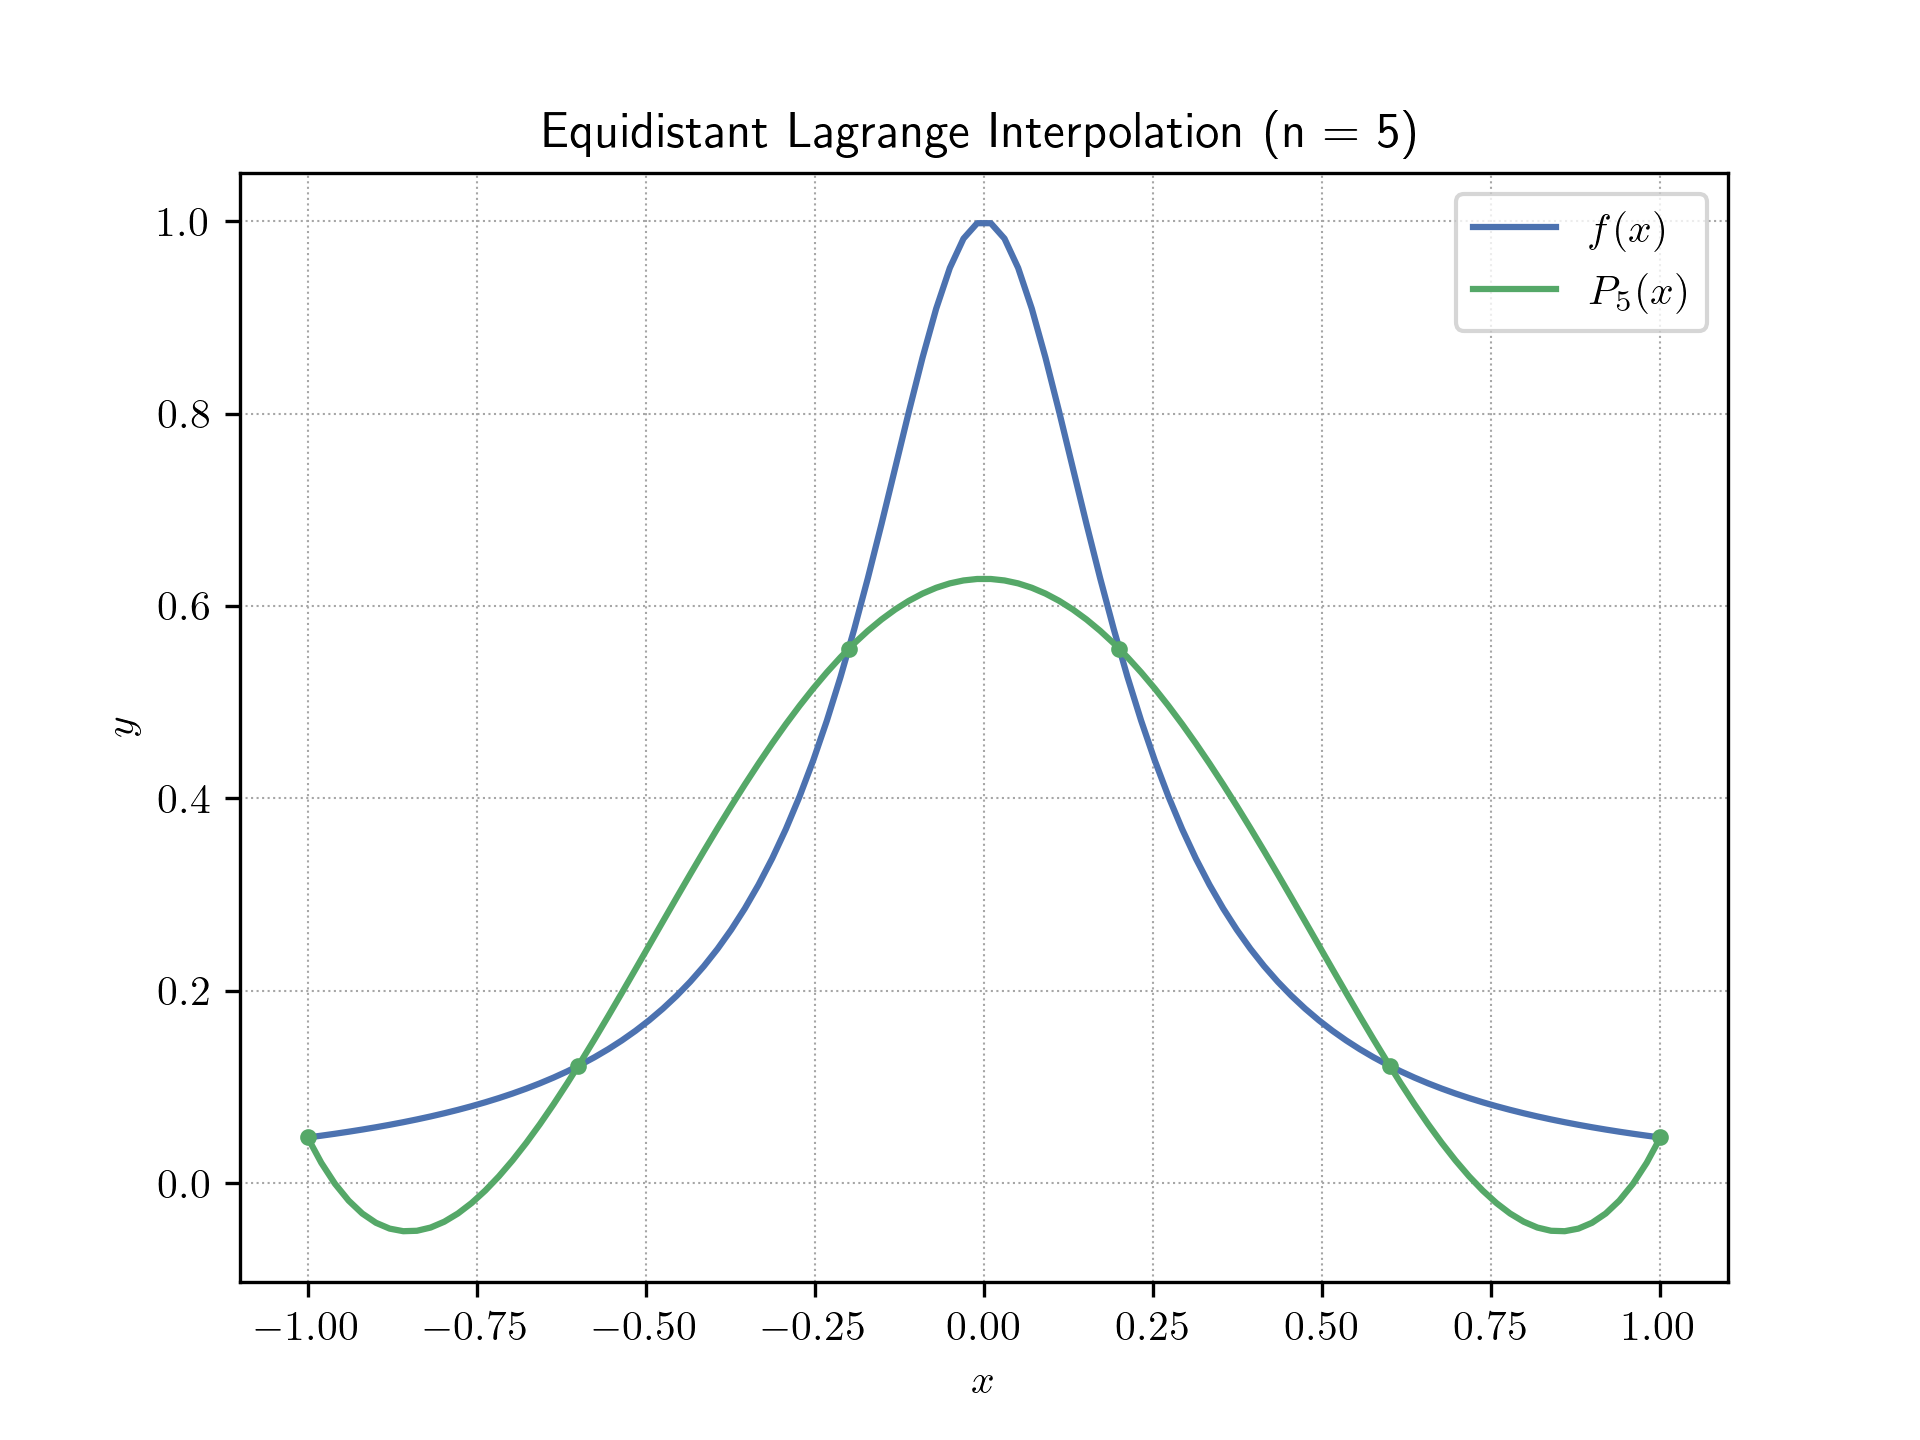
\includegraphics[width=0.8\textwidth]{../plots_2/q2_2/p5.png}
    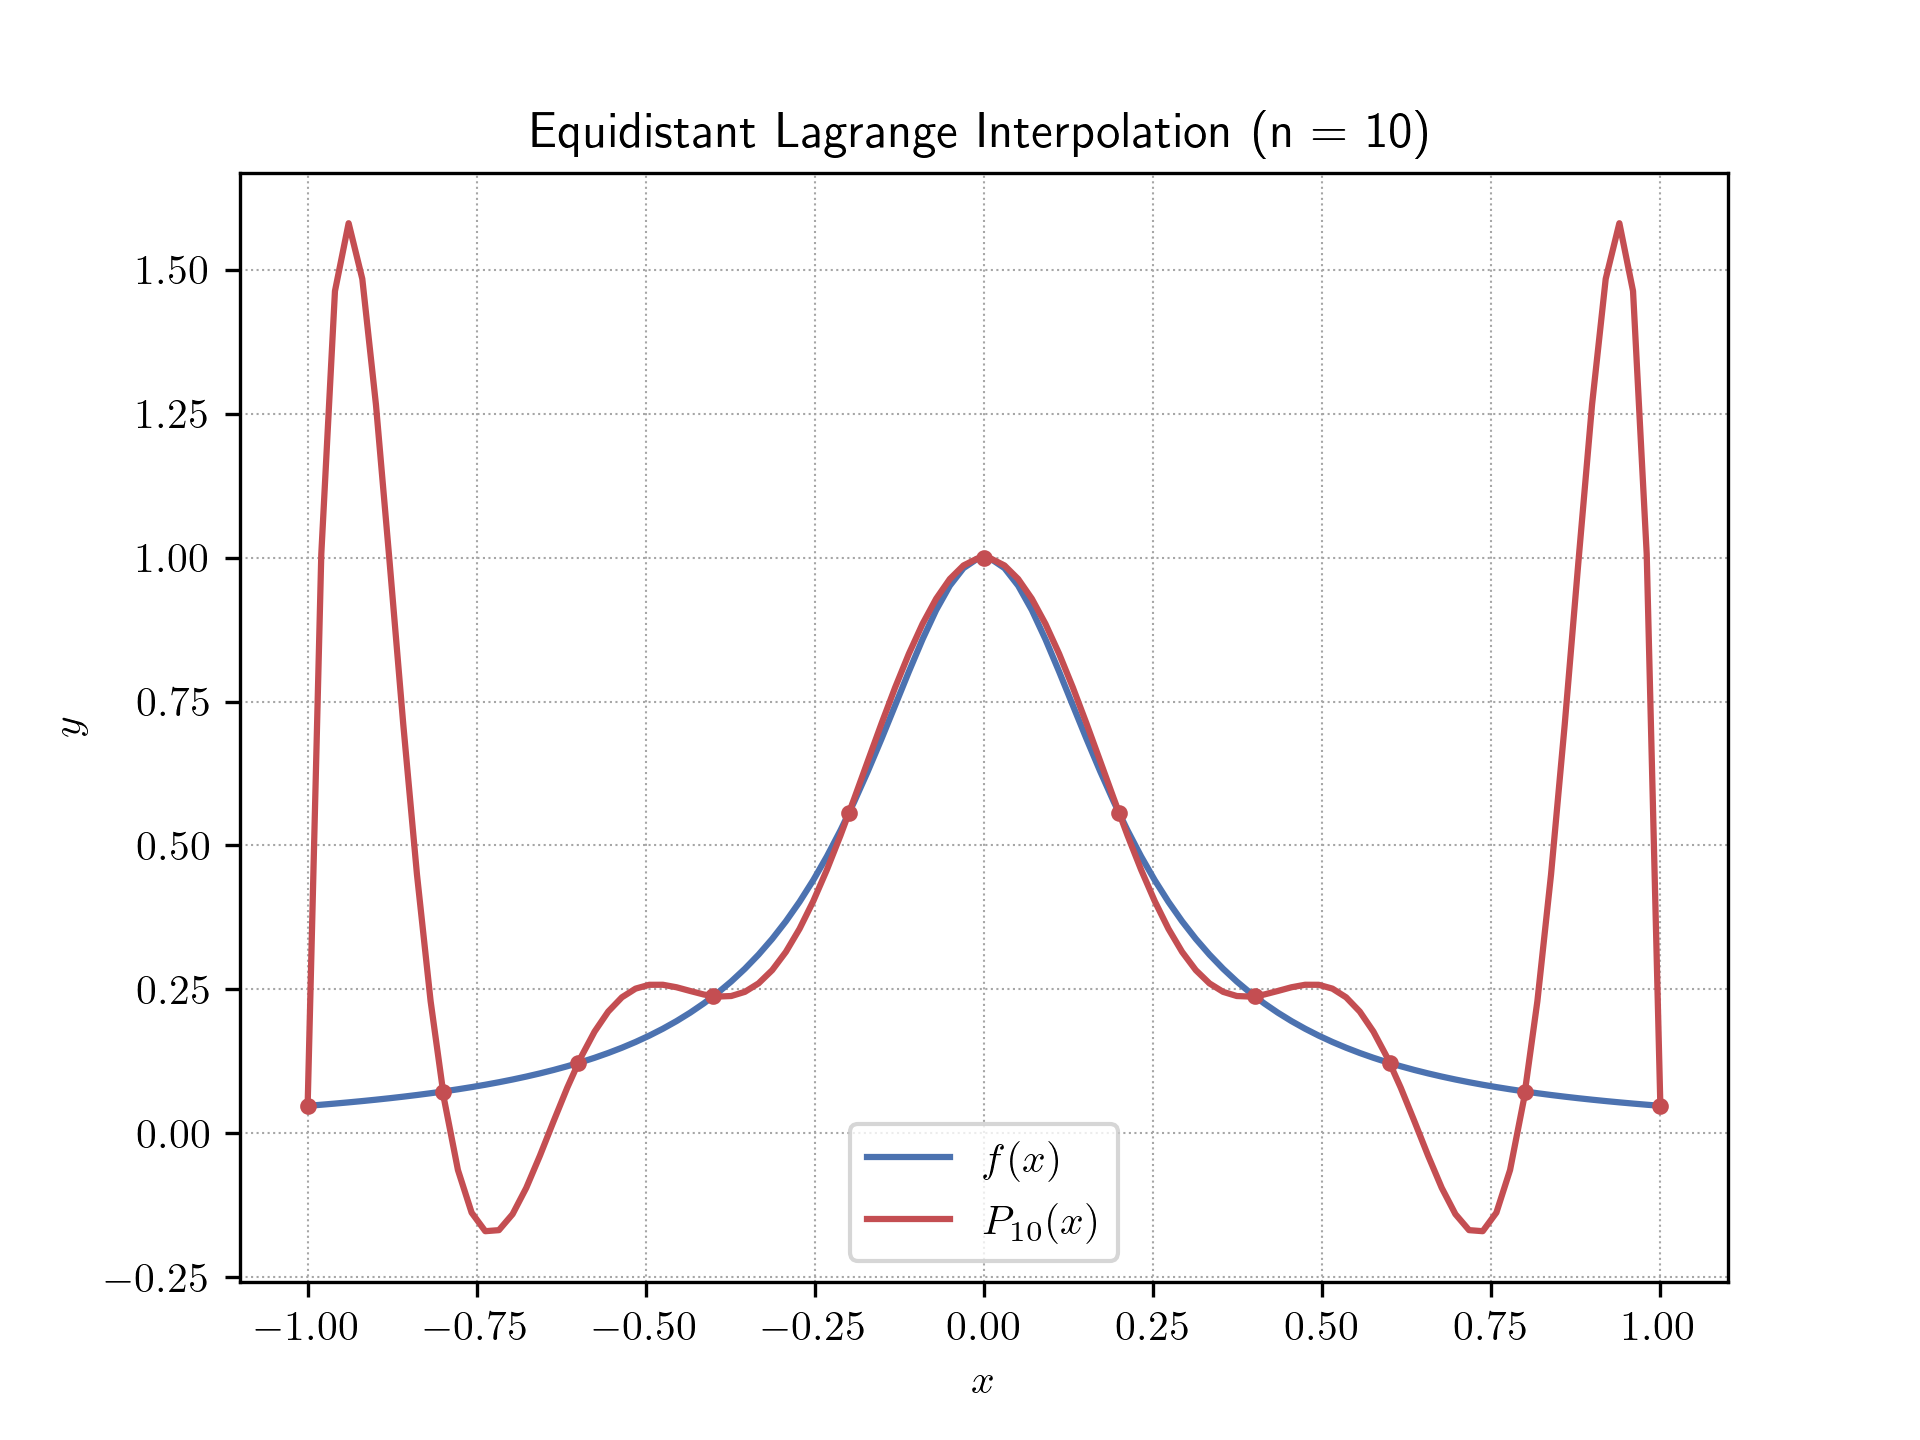
\includegraphics[width=0.8\textwidth]{../plots_2/q2_2/p10.png}
    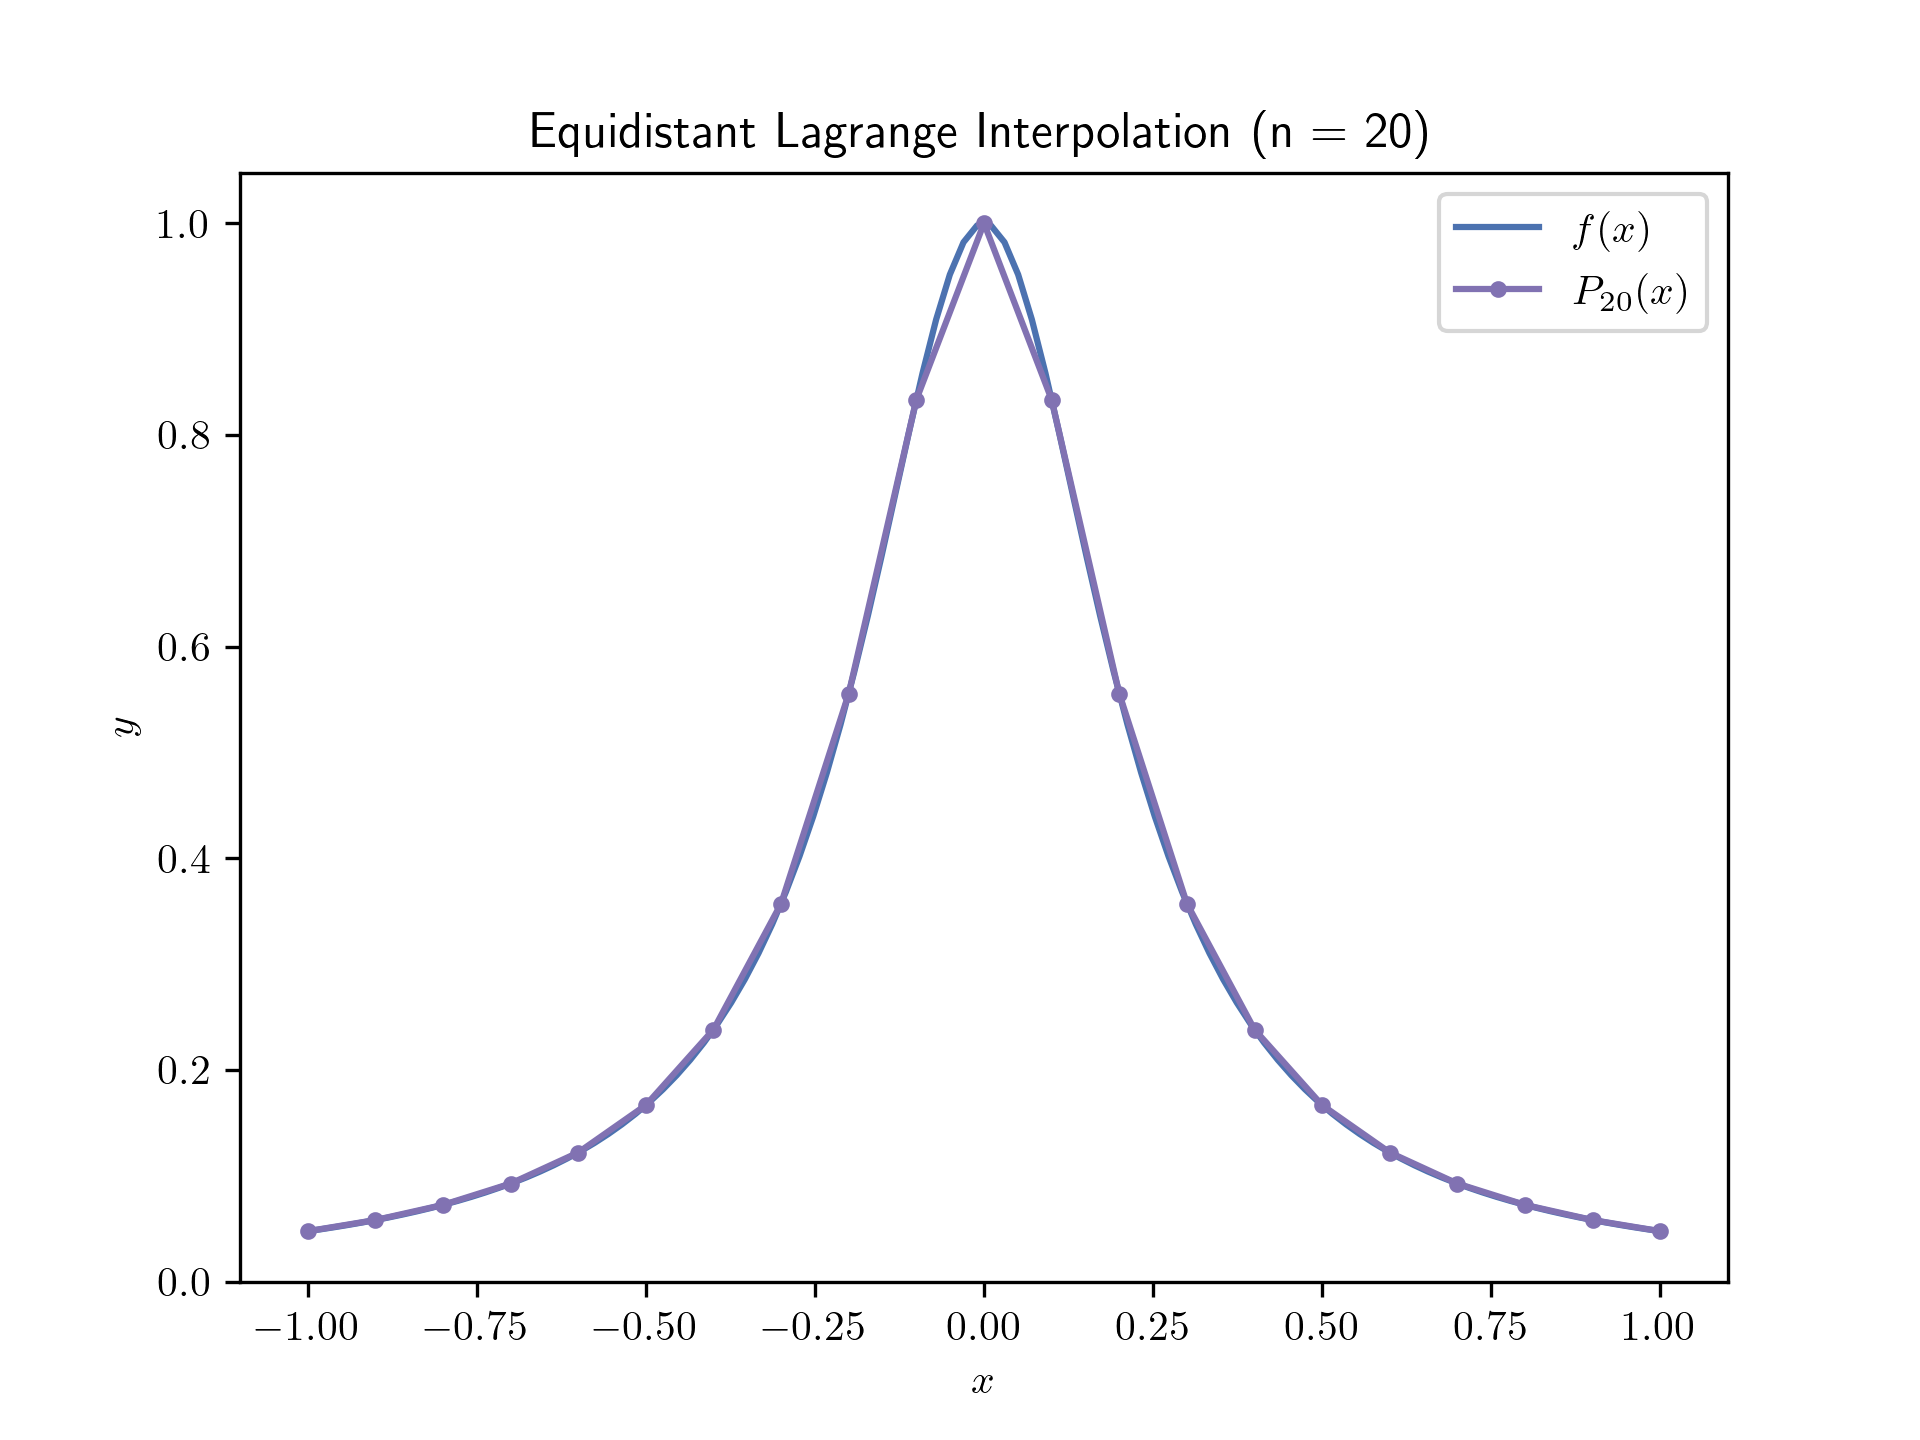
\includegraphics[width=0.8\textwidth]{../plots_2/q2_2/p20.png}
    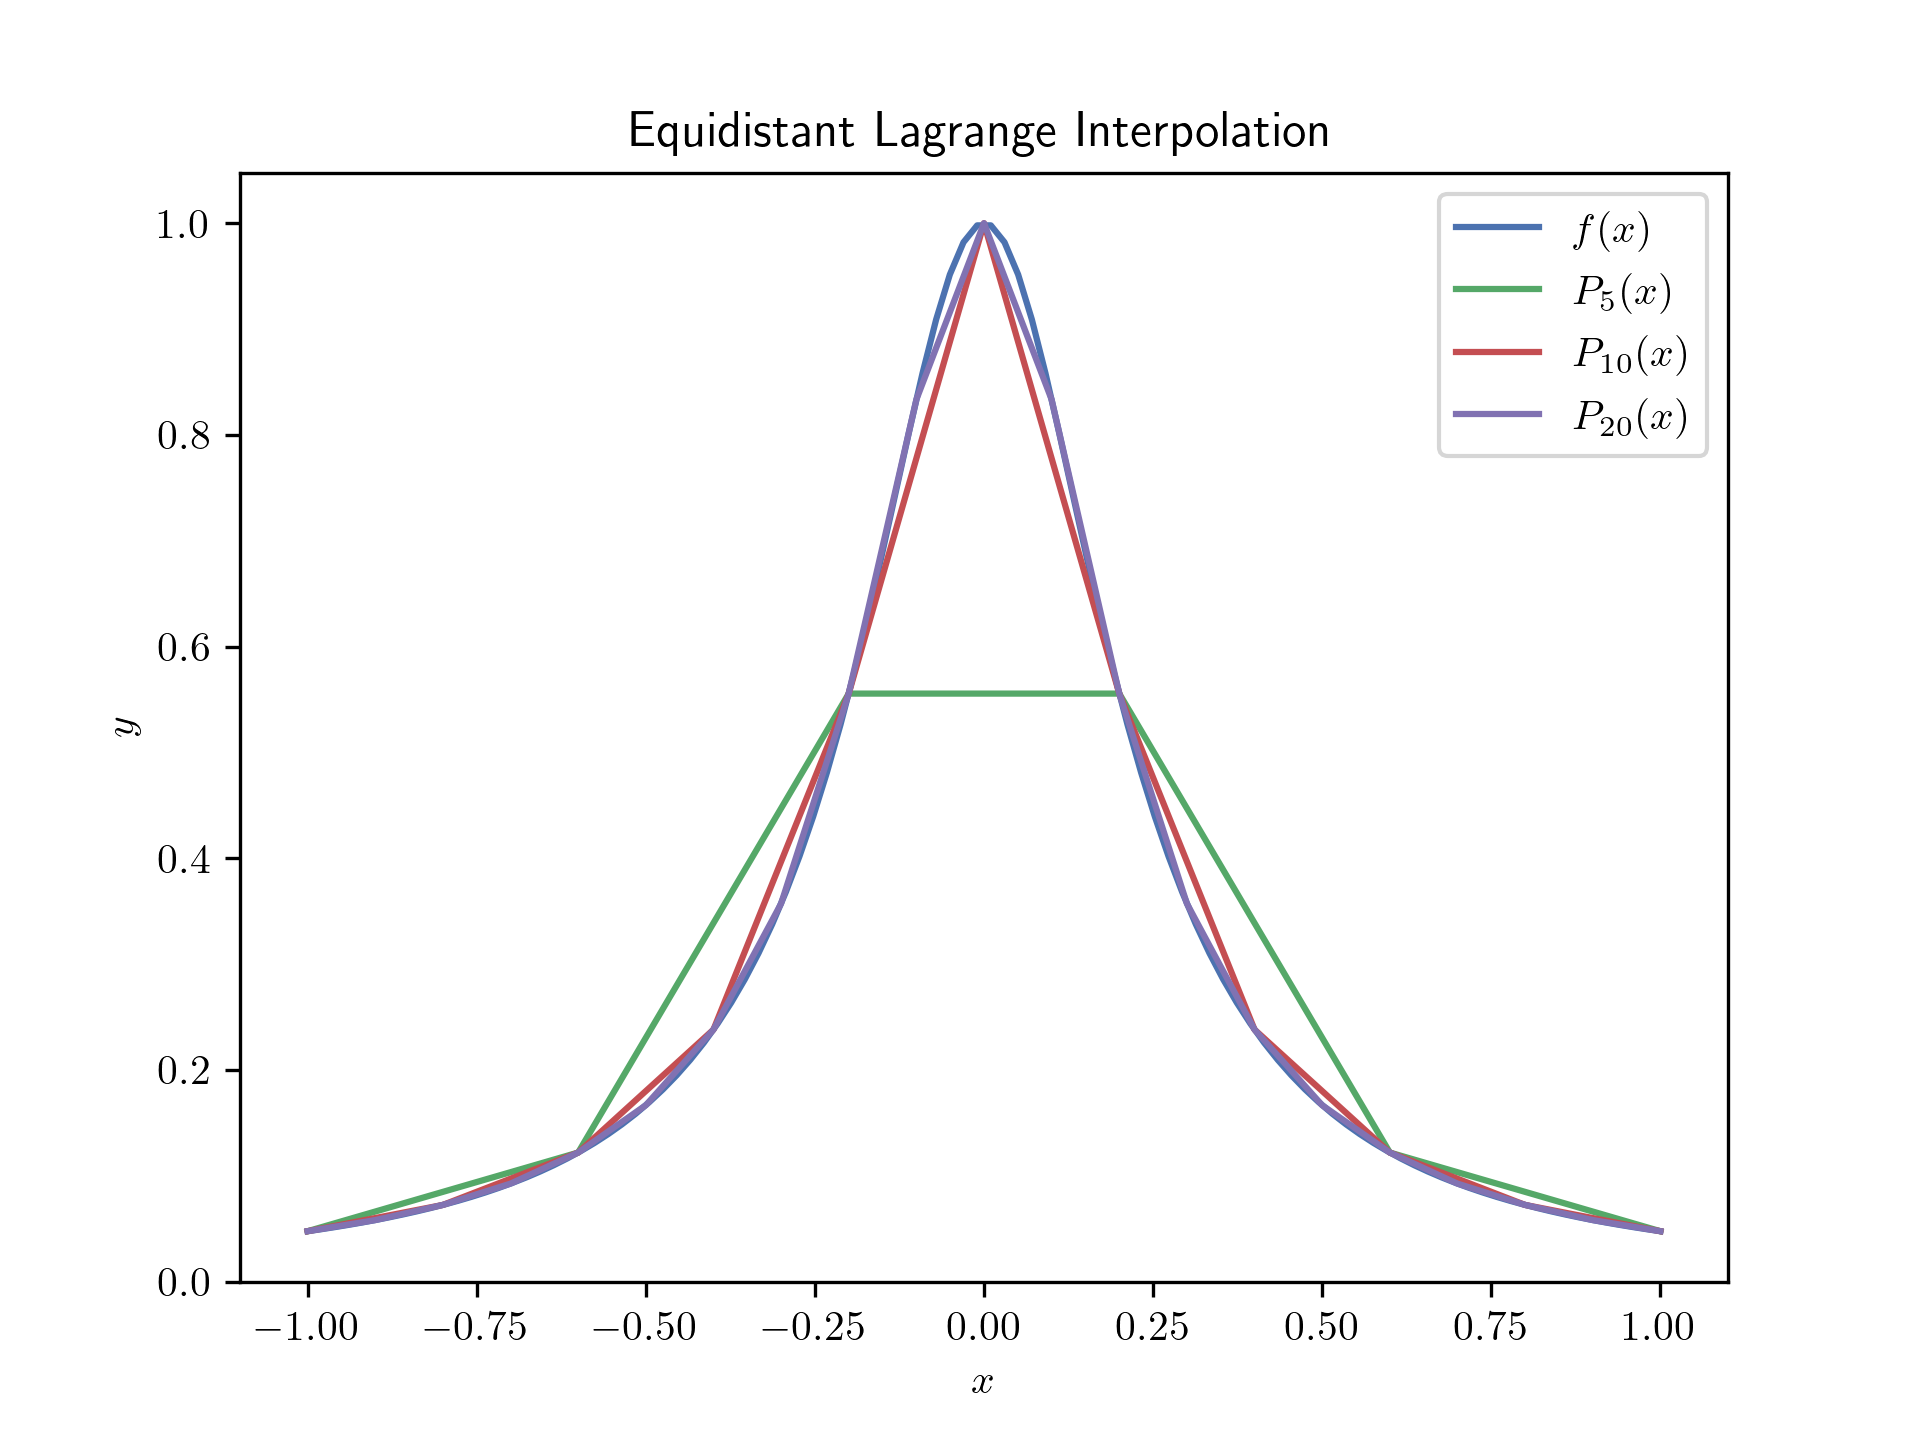
\includegraphics[width=0.8\textwidth]{../plots_2/q2_2/all.png}
\end{center}

As $n$ increases from $5$ to $10$ and $20$, we see that the interpolation error decreases towards the center of the interval $[-1,1]$. However, the error increases significantly near the edges of the interval, demonstrating Runge's phenomenon. 

\newpage
\subquestion
Repeat the interpolation using Chebyshev nodes, and compare the results with the equidistant-node case.

\solution
In addition to the functions defined in the previous parts, the following function was used to generate the Chebyshev nodes:
\begin{lstlisting}[language=Python, caption=2.3 Python]
import math
import numpy as np

def chebyshev_nodes(n):
    nodes = np.array(
        [(math.cos((2 * k - 1) * math.pi / (2 * n))) for k in range(1, n + 1)]
    )

    return nodes

# The main method is almost identical to the previous part.
# The only difference is that chebyshev_nodes(n[i] + 1) 
# is used instead of np.linspace(-1, 1, n[i] + 1) to generate the nodes.
\end{lstlisting}

Th following plots show $f(x)$ and $P_n(x)$ for Chebyshev nodes with $n=5, 10, 20$:
\begin{center}
    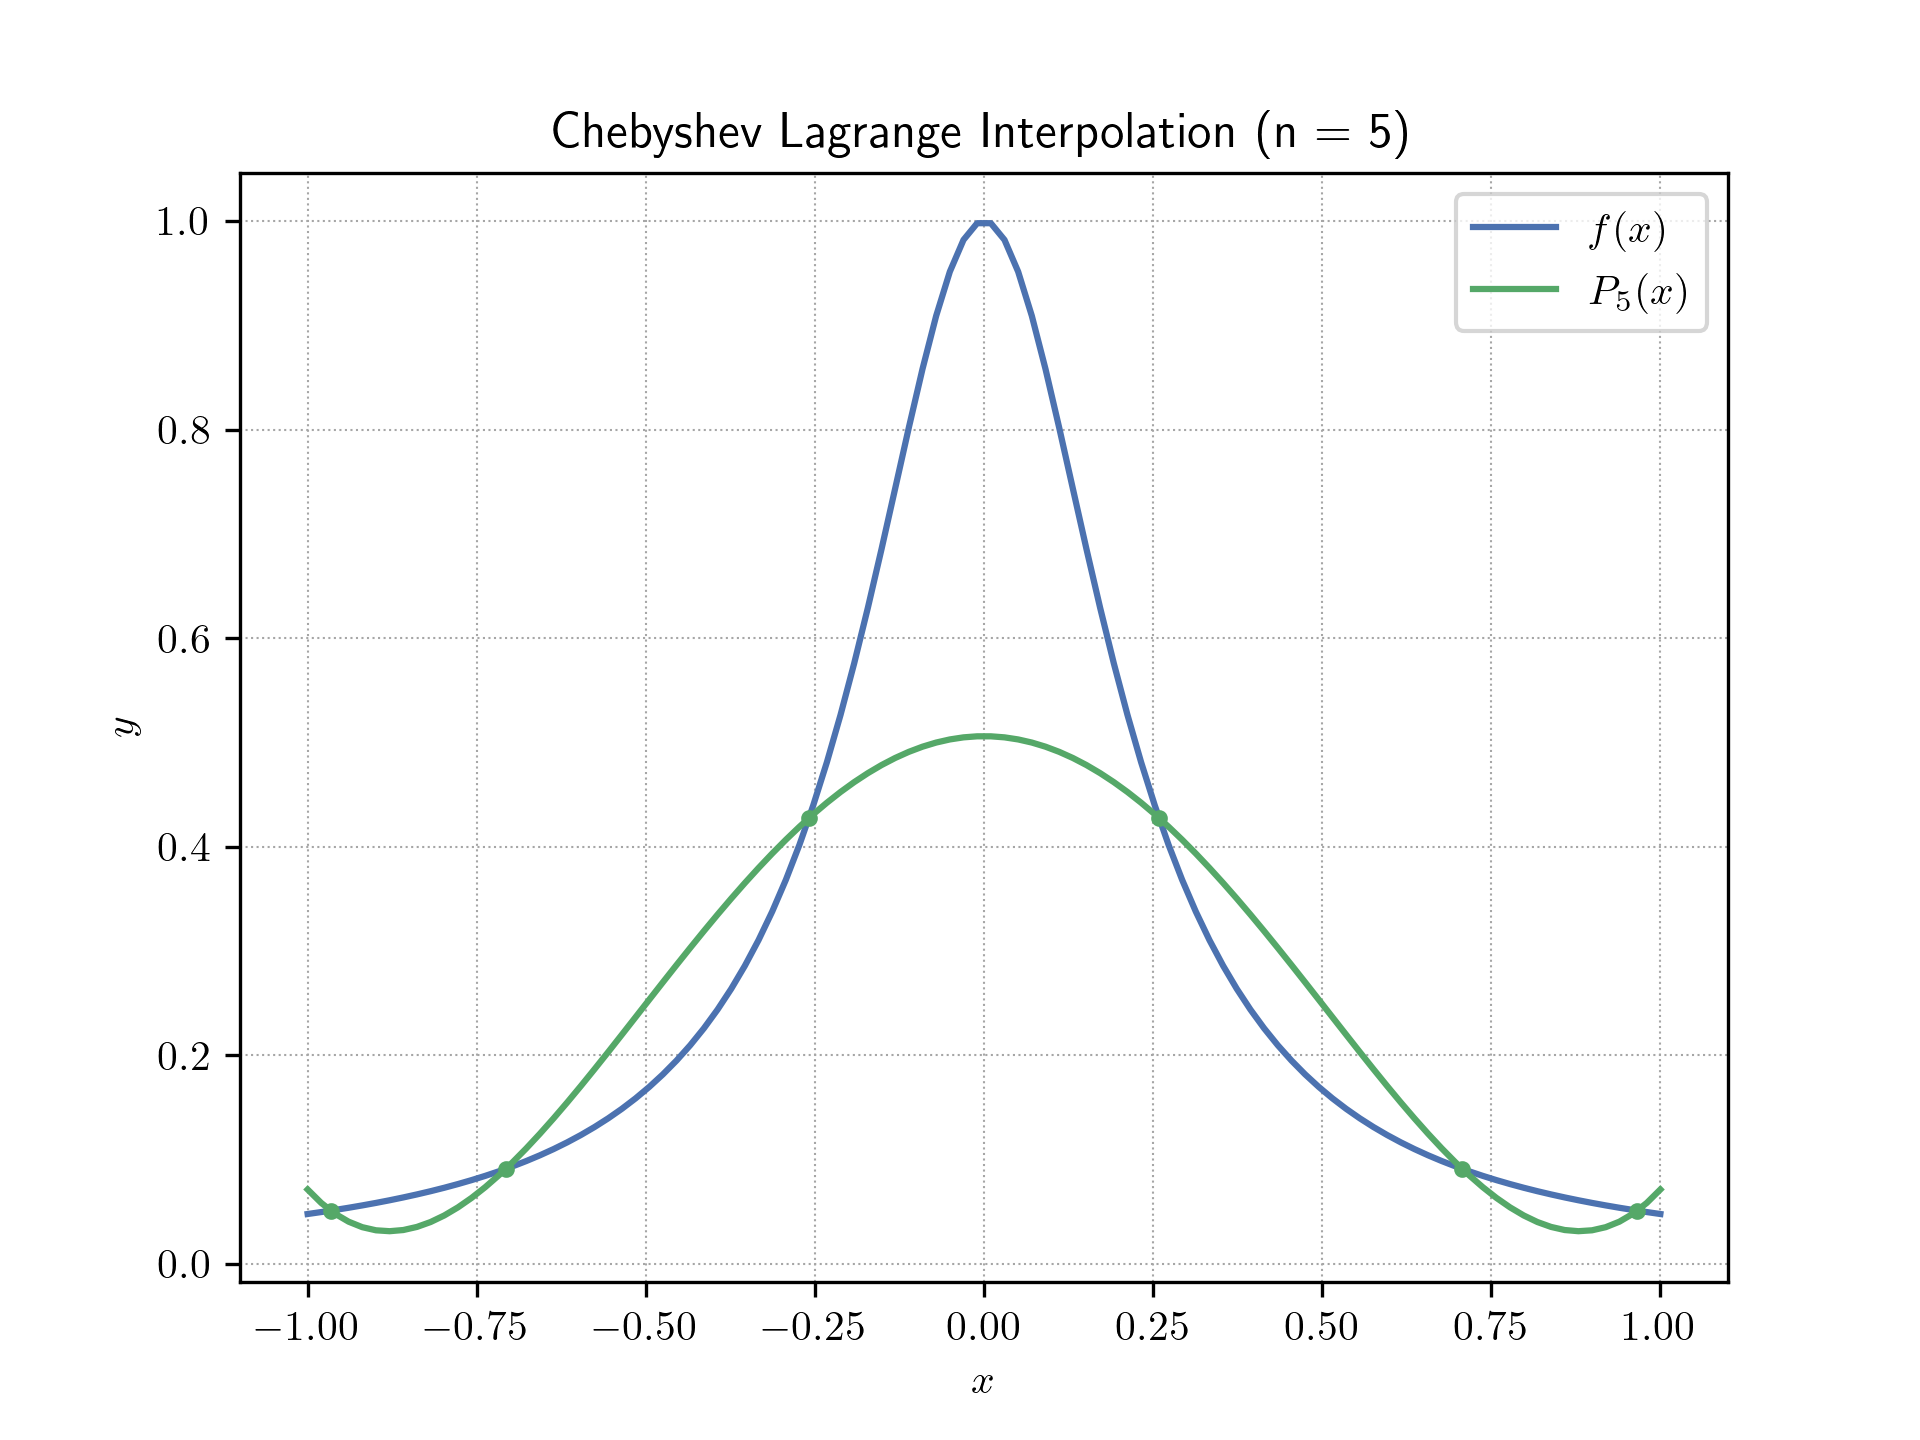
\includegraphics[width=0.8\textwidth]{../plots_2/q2_3/chebyshev_p5.png}
    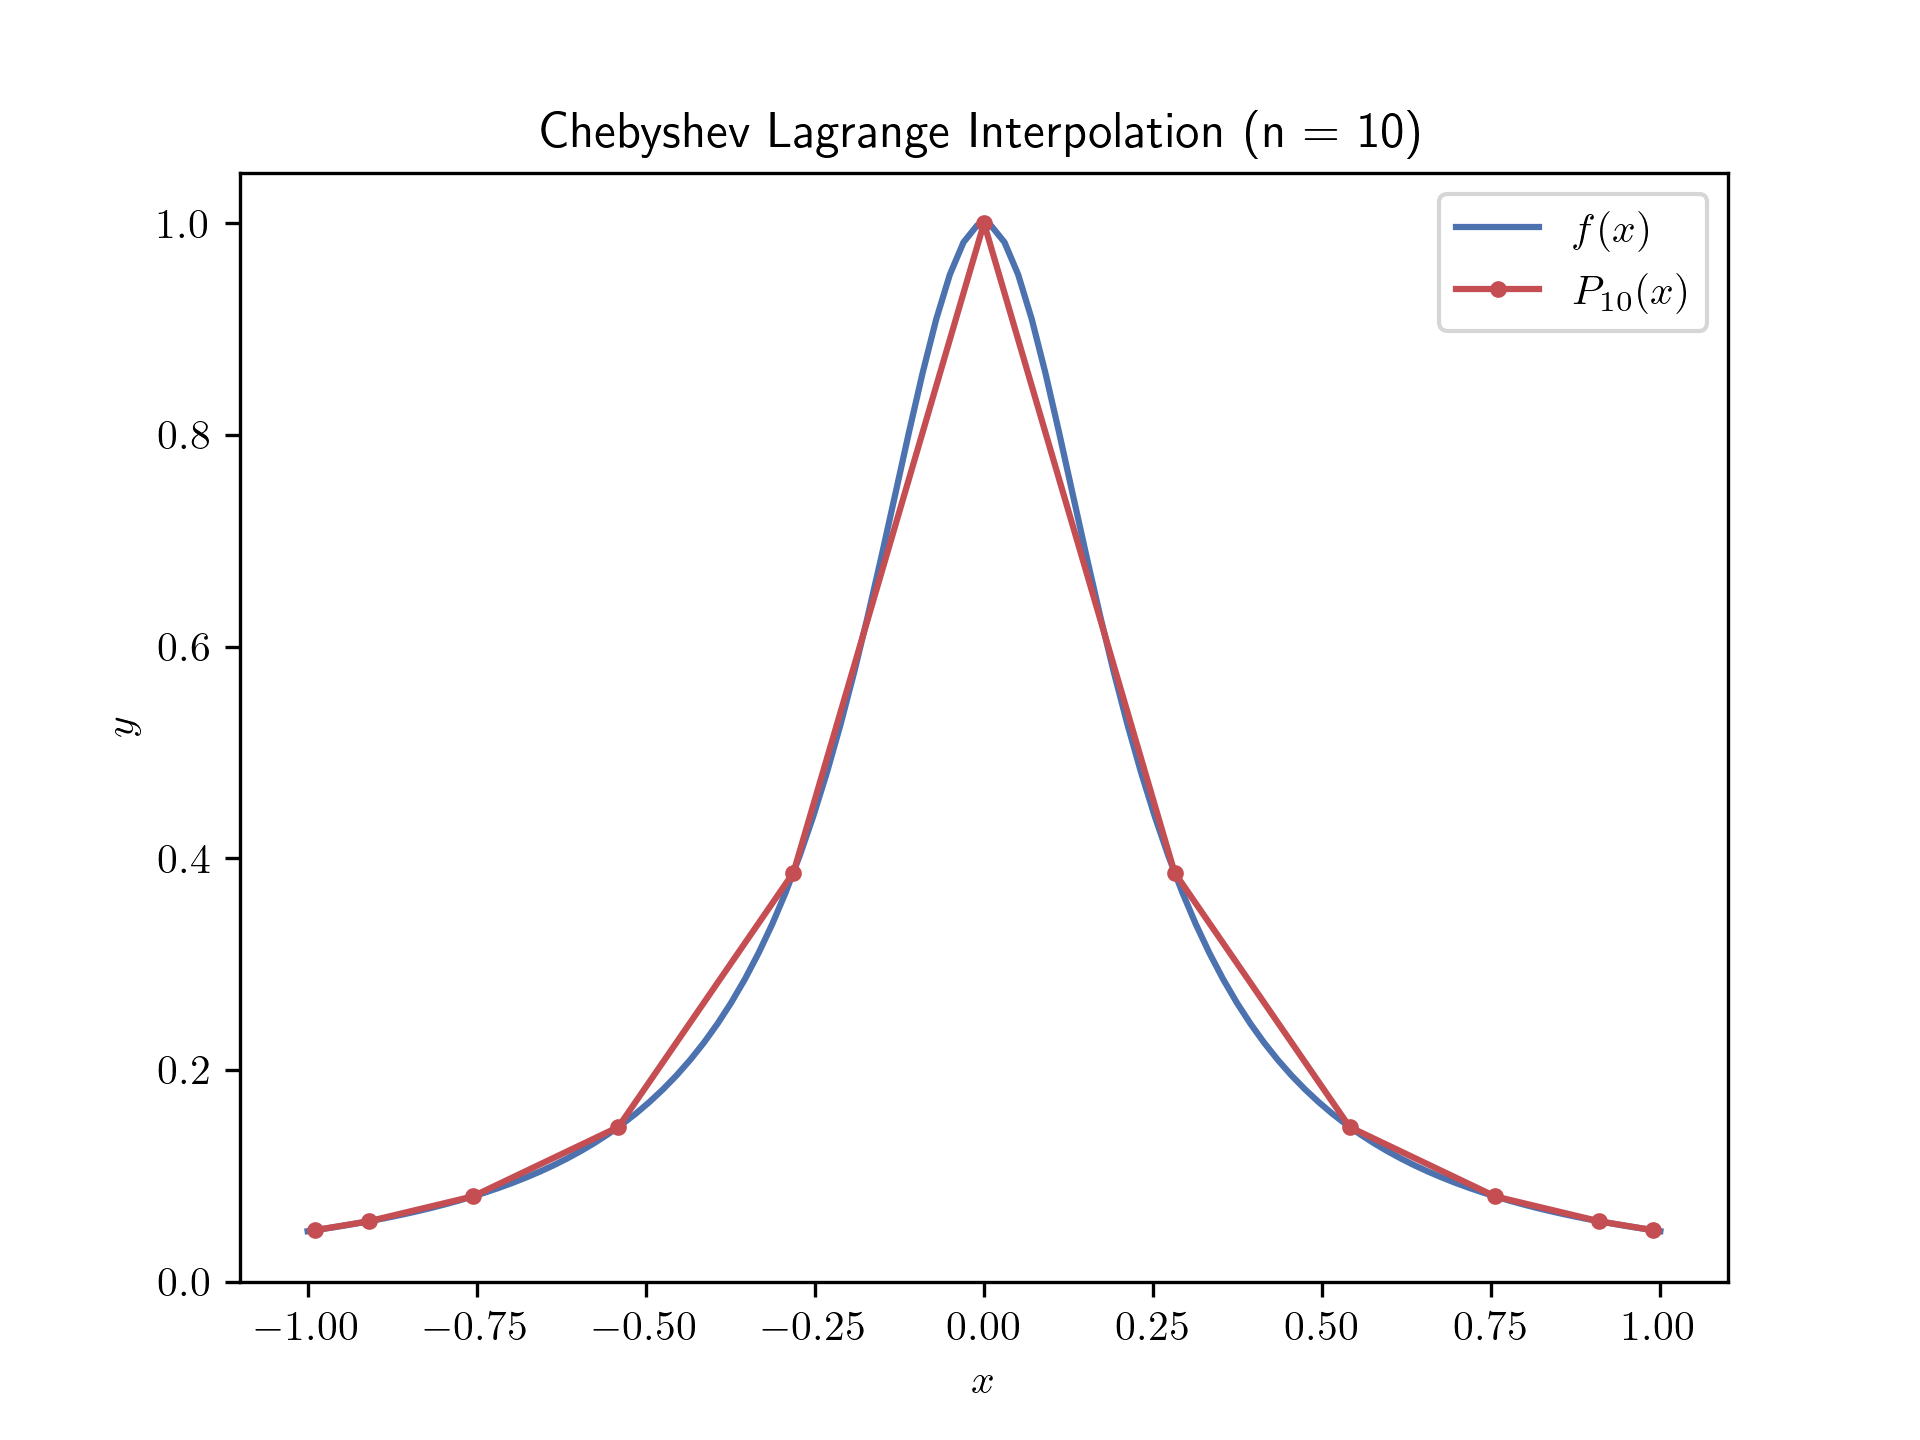
\includegraphics[width=0.8\textwidth]{../plots_2/q2_3/chebyshev_p10.png}
    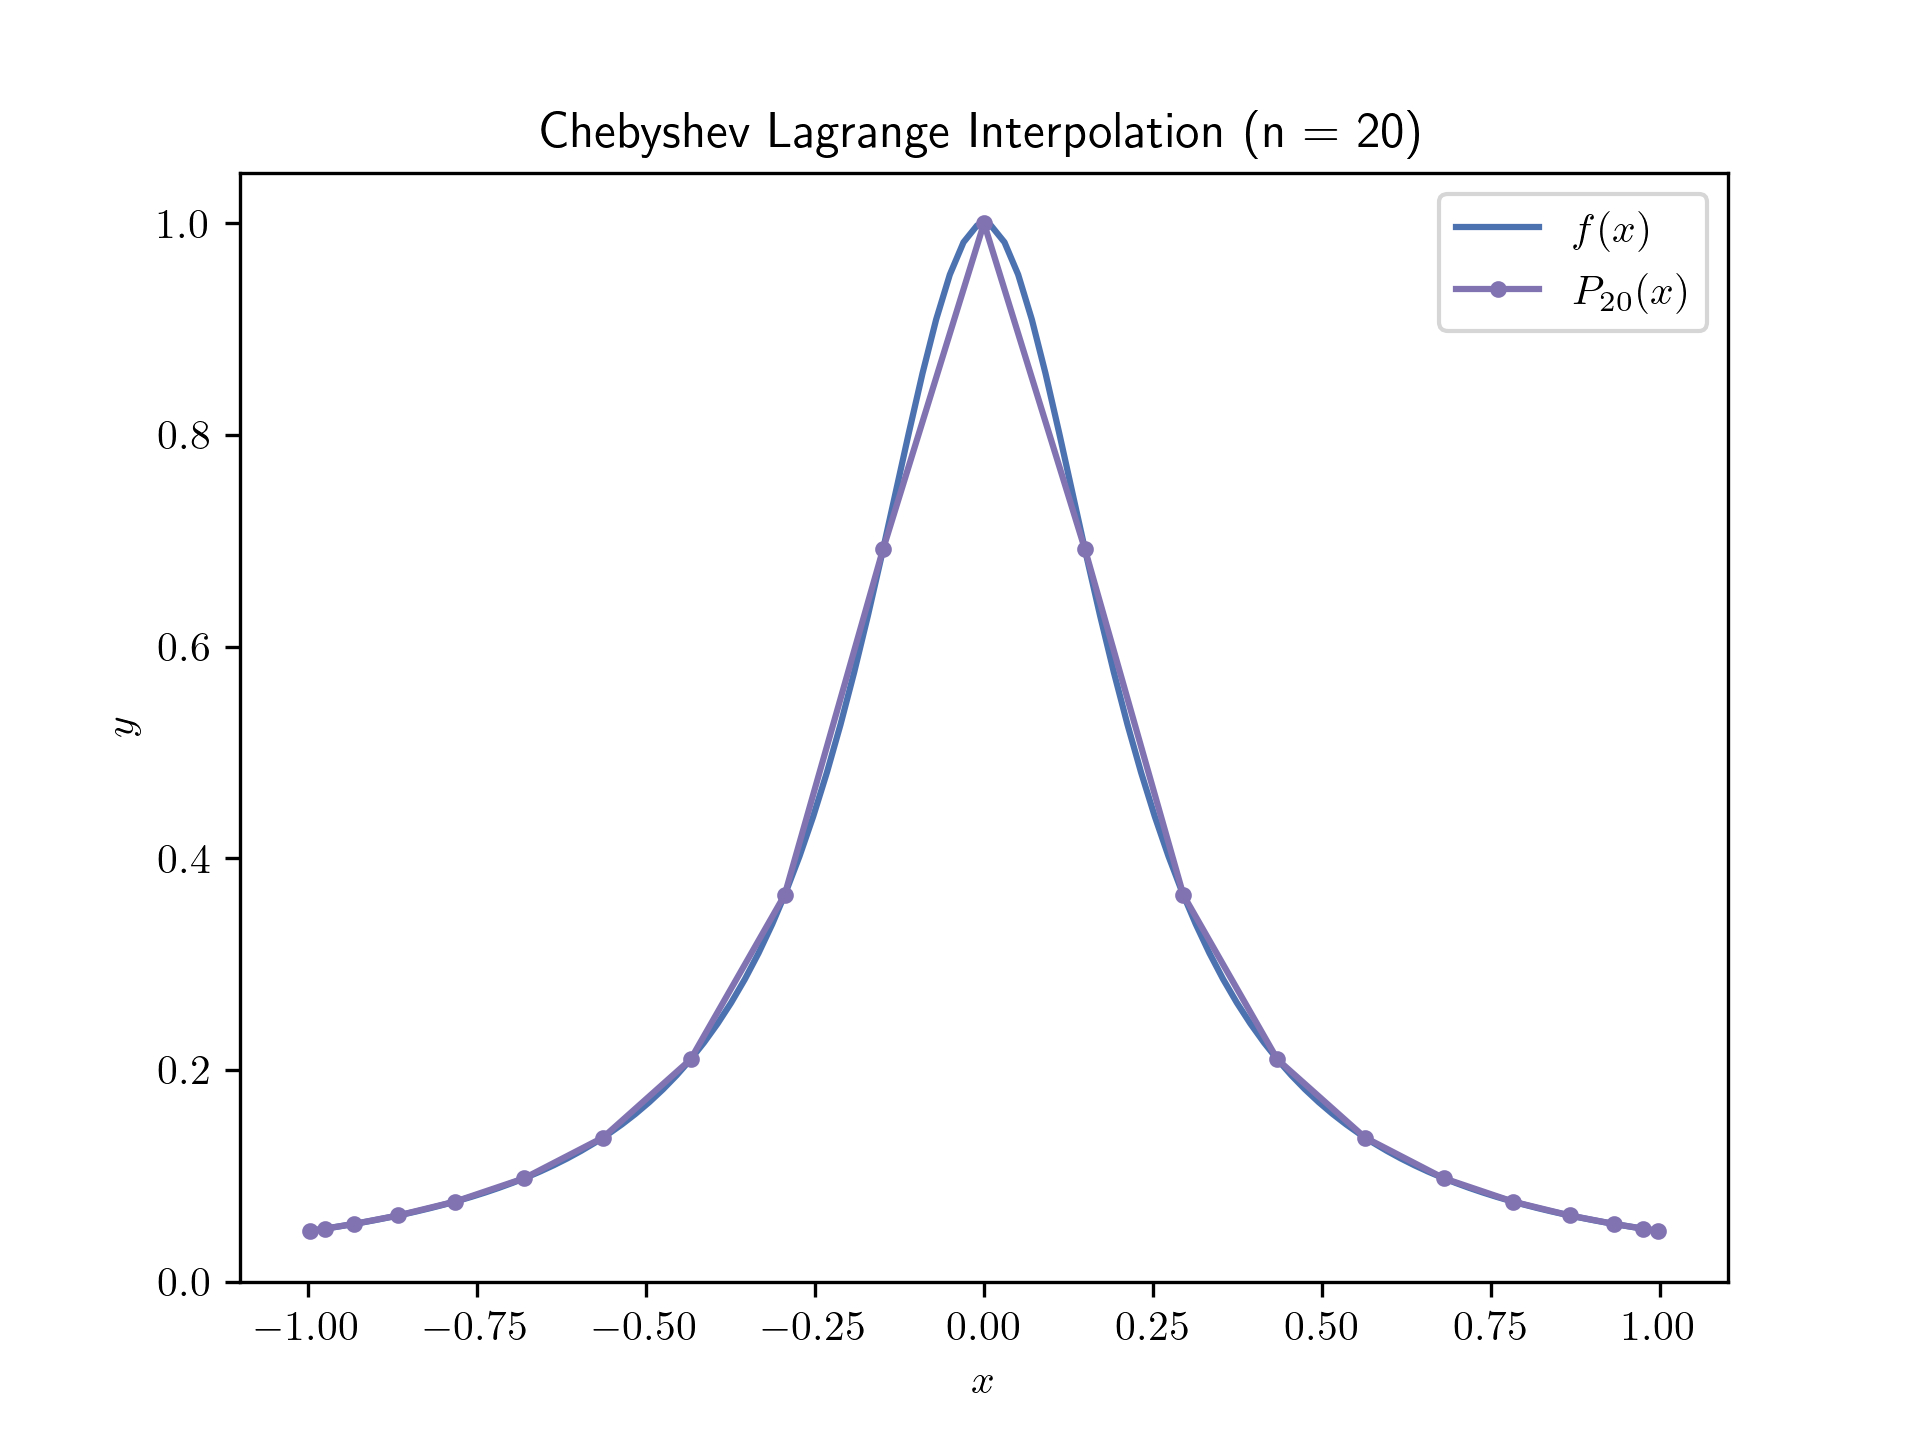
\includegraphics[width=0.8\textwidth]{../plots_2/q2_3/chebyshev_p20.png}
    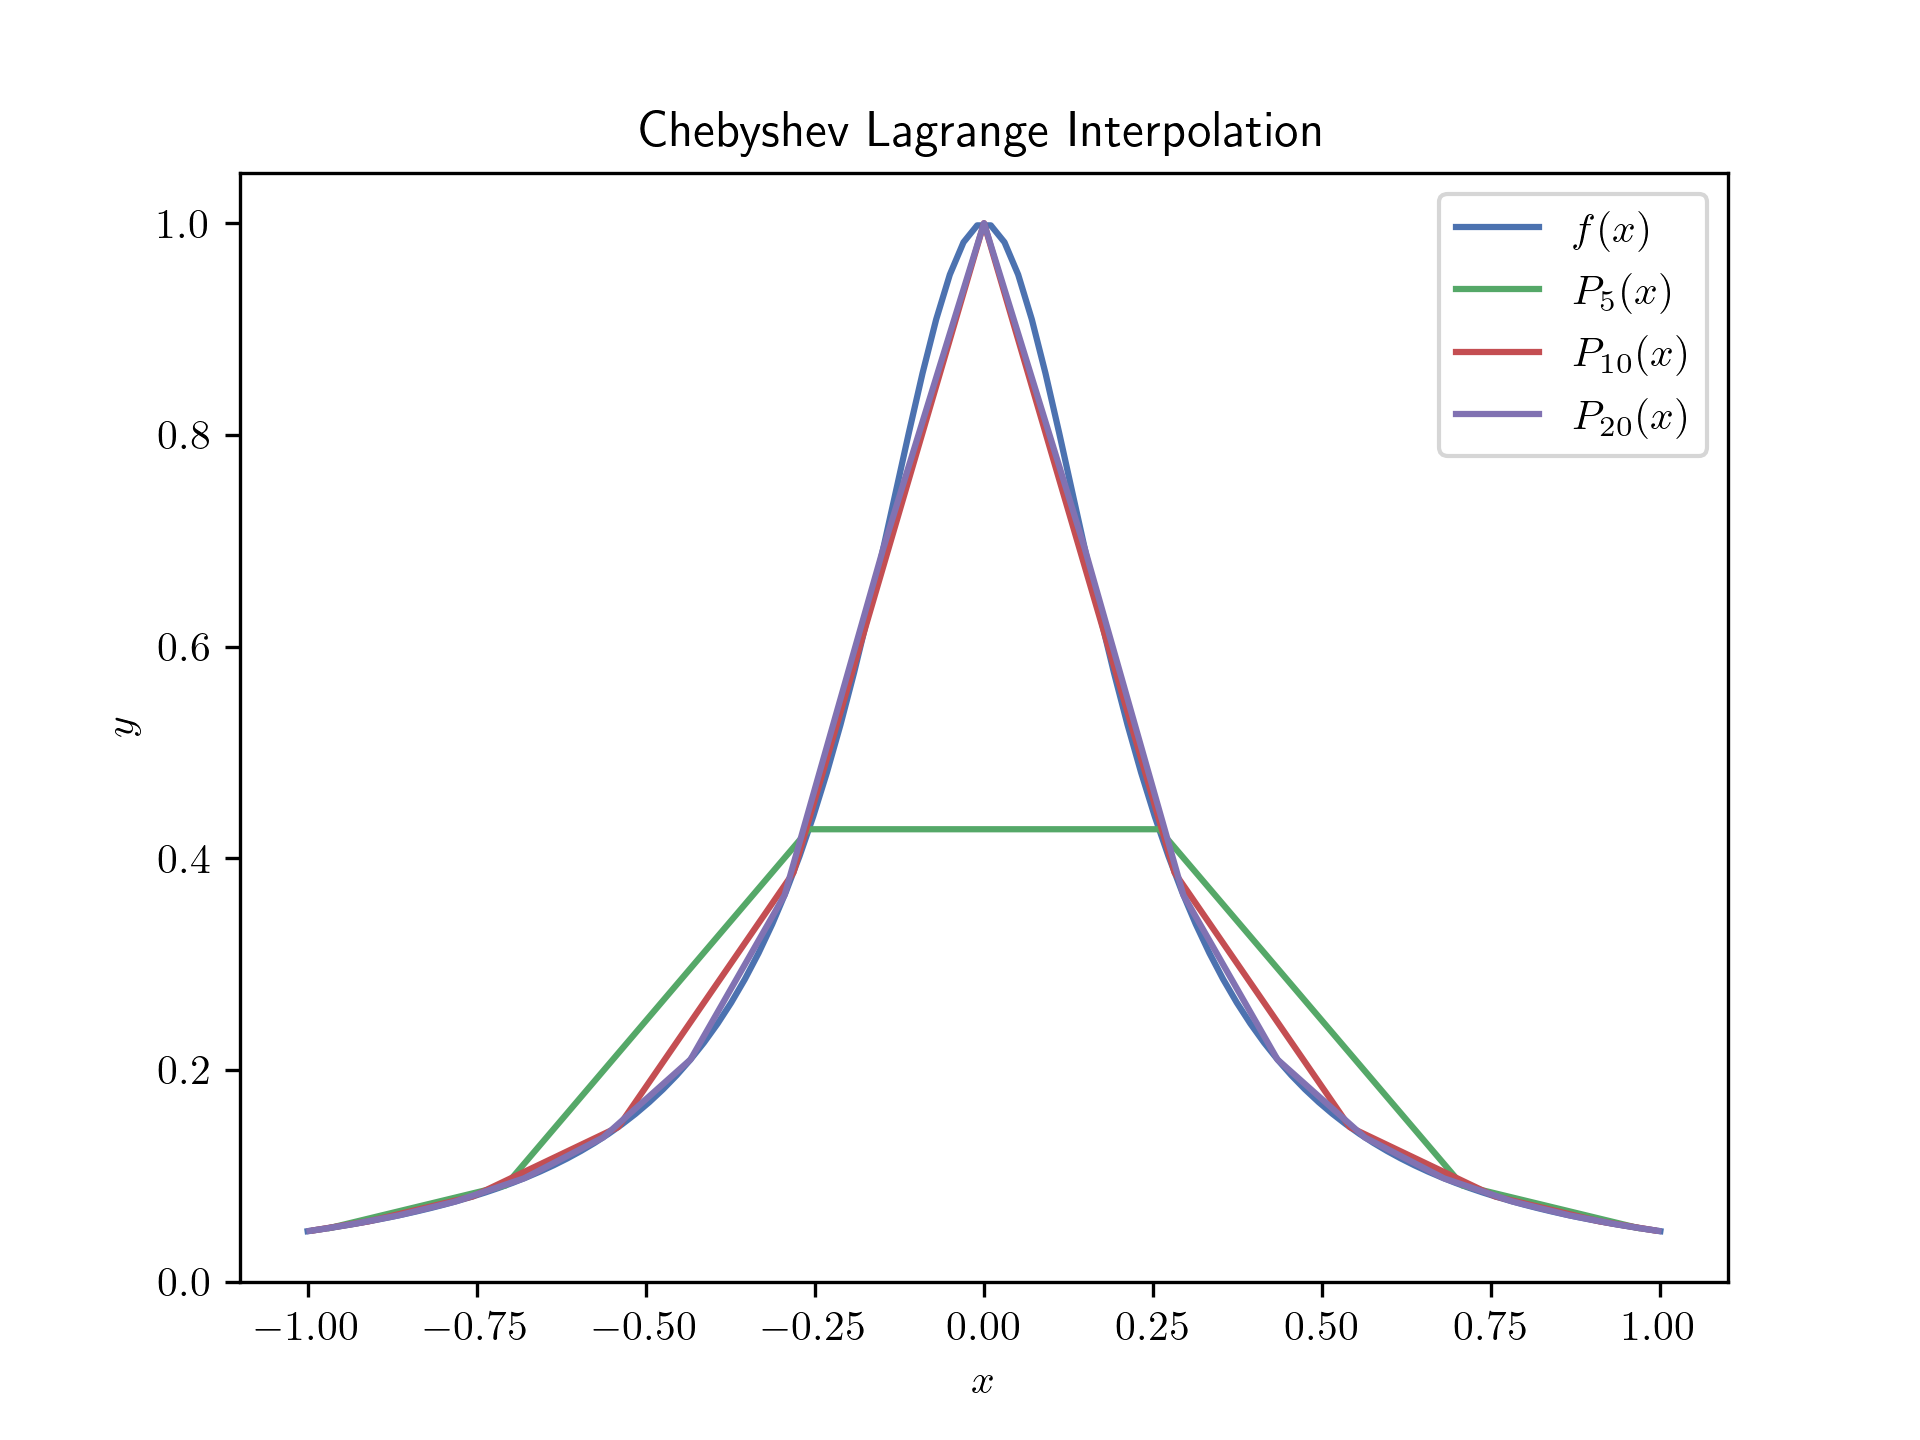
\includegraphics[width=0.8\textwidth]{../plots_2/q2_3/chebyshev_all.png}
\end{center}

Comparing these plots to those with equidistant nodes, we see that using Chebyshev nodes significantly reduces the interpolation error across the entire interval $[-1,1]$. The oscillations near the edges of the interval are much less pronounced, demonstrating that Chebyshev nodes help mitigate Runge's phenomenon and provide a more accurate approximation of $f(x)$.

\newpage
\question{Chebyshev Polynomials and Their Roots}
The Chebyshev polynomials of the first kind is defined by:
\[T_n(x) = \cos(n \arccos x), \quad x \in [-1,1]\]

\subquestion
Prove that the numbers
\[x_k = \cos\left(\frac{2k-1}{2n} \pi\right), \quad k=1,2,\dots,n\]
are the roots of $T_n(x)$.

\begin{proof}
    We want to find the values of $x$ such that $T_n(x) = 0$. By the definition of Chebyshev polynomials, we have:
    \[T_n(x) = \cos(n \arccos x)\]
    Setting $T_n(x) = 0$, we get:
    \[T_n(x) = \cos(n \arccos x) = 0\]
    The cosine function is zero at odd multiples of $\frac{\pi}{2}$.
    So $T_n(x)$ can only equal zero when $n \arccos x$ is an odd multiple of $\frac{\pi}{2}$. Therefore, we can write:
    \[n \arccos x = \frac{(2k-1)\pi}{2}, \quad k \in \mathbb{Z}\]
    Note that for $n=0$, $T_0(x) = \cos(0\cdot \arccos(x))=1$ which has no roots. So consider $n \geq 1$. Dividing both sides by $n$, we have:
    \[\arccos x = \frac{(2k-1)\pi}{2n}, \quad k \in \mathbb{Z}\]
    Taking the cosine of both sides, we get:
    \[x = \cos\left(\frac{(2k-1)\pi}{2n}\right), \quad k \in \mathbb{Z}\]
    Therefore, the set of x defined above are the roots of $T_n(x)$ for $n\geq 1$. Note that if we restrict $k$ to the integers $1, 2, \dots, n$, we exactly get that:
    \[x_k = \cos\left(\frac{2k-1}{2n} \pi\right), \quad k=1,2,\dots,n\]
    are the roots of $T_n(x)$.
\end{proof}

\newpage
\subquestion
Show that these roots are distinct and lie in the interval $(-1,1)$.

\begin{proof}
    To show that these roots are distinct, we need to show that for $k_1 \neq k_2$, we have $x_{k_1} \neq x_{k_2}$. Assume $k_1, k_2 \in \{1, 2, \dots, n\}$ such that $k_1 \neq k_2$ and $k_1 < k_2$. Then, assuming for fixed $n\geq 1$:
    \[x_{k_1} = \cos\left(\frac{2k_1-1}{2n} \pi\right), \quad 
    x_{k_2} = \cos\left(\frac{2k_2-1}{2n} \pi\right)\]
    Note that $\frac{2k_1-1}{2n} \pi$ and $\frac{2k_2-1}{2n} \pi$ are distinct angles in the interval $(0, \pi)$.
    Since the cosine function is strictly decreasing on the interval    $[0, \pi]$, and since $\frac{2k_1-1}{2n} \pi < \frac{2k_2-1}{2n} \pi$ are distinct, we have:
    \[x_{k_1} = \cos\left(\frac{2k_1-1}{2n} \pi\right) > \cos\left(\frac{2k_2-1}{2n} \pi\right) = x_{k_2}\]
    By the law of trichotomy, $x_{k_1} \neq x_{k_2}$. Therefore, the roots $x_k$ are distinct for $k=1, 2, \dots, n$.

    Next, we need to show that these roots lie in the interval $(-1,1)$. Note that from above, we have shown that ${x_k}$ is a strictly decreasing sequence. Therefore, we only need to show that the largest root $x_1$ is less than $1$ and the smallest root $x_n$ is greater than $-1$.

    First, let us show that $x_1 < 1$:
    \[x_1 = \cos\left(\frac{2(1)-1}{2n} \pi\right) = \cos\left(\frac{\pi}{2n}\right)\]
    Note that $\frac{\pi}{2n} \in (0, \frac{\pi}{2}]$. In this interval, the range of the cosine function is $[0,1)$. Therefore, we have:
    \[x_1 = \cos\left(\frac{\pi}{2n}\right) < 1 \label{x1}\tag{1}\]   
    Next, let us show that $x_n > -1$:
    \[x_n = \cos\left(\frac{2n-1}{2n} \pi\right) = \cos\left(\pi - \frac{\pi}{2n}\right)\]
    Note that $\pi - \frac{\pi}{2n} \in [\frac{\pi}{2}, \pi)$. In this interval, the range of the cosine function is $(-1, 0]$. Therefore, we have:
    \[x_n = \cos\left(\pi - \frac{\pi}{2n}\right) > -1 \label{xn}\tag{2}\]
    Combining \eqref{x1} and \eqref{xn}, we have shown that:
    \[-1 < x_n < x_k < x_1 < 1\]
    Therefore, $x_k$ are distinct roots that lie in the interval $(-1,1)$ for $k=1, 2, \dots, n$.
\end{proof}

\newpage
\subquestion
Write your own code to generate $T_n(x)$ using the recursion formula.

\solution The following code was used to generate the Chebyshev polynomials::
\begin{lstlisting}[language=Python, caption=3.3 Python]
import sympy as smp

def chebyshev_poly(n):
    # Base Cases
    if n == 0:
        return 1
    elif n == 1:
        return smp.symbols("x")
    # Recursive Case
    else:
        return 2 * smp.symbols('x') * chebyshev_poly(n - 1) - chebyshev_poly(n - 2)

def generate_chebyshev(n):
    x = smp.symbols('x')
    poly = smp.expand(chebyshev_poly(n))
    function = f"T_{{{n}}}({x})"
    equation = function + " = " + smp.latex(poly) 
    return equation, poly

# Main Method
if __name__ == "__main__":
# Used for plotting in next part
polys = []

# Generate and save equations to a text file
with open("./plots_2/q3_3/chebyshev_polynomials.txt", "w") as file:
    for n in range(6):
        equation, poly = generate_chebyshev(n)
        polys.append(poly)
        file.write(equation + "\n")
\end{lstlisting}

The Chebyshev polynomials $T_n(x)$ for $n=0, 1, \dots, 5$ are given by:
\begin{align*}
    T_{0}(x) &= 1 \\
    T_{1}(x) &= x \\
    T_{2}(x) &= 2 x^{2} - 1 \\
    T_{3}(x) &= 4 x^{3} - 3 x \\
    T_{4}(x) &= 8 x^{4} - 8 x^{2} + 1 \\
    T_{5}(x) &= 16 x^{5 }- 20 x^{3} + 5 x \\
\end{align*}

\subquestion
Plot the first six polynomials $T_0(x), T_1(x), \dots, T_5(x)$ on the interval $[-1,1]$.

\solution The following code was used to plot the Chebyshev polynomials:
\begin{lstlisting}[language=Python, caption=3.4 Python]
import numpy as np
import matplotlib.pyplot as plt
import sympy as smp

if __name__ == "__main__":
    # <some matplotlib styling>
    # polys list was generated in previous part
    x_coords = np.linspace(-1, 1, 100)
    x = smp.symbols("x")

    fig, ax = plt.subplots()
    # Plot each polynomial
    for i in range(6):
        # Evaluate polynomial at each x coordinate
        if i != 0:
            y_coords = np.array(
                [polys[i].evalf(subs={x: x_coords[j]}) for j in range(len(x_coords))]
            )
        # Case for T_0(x) = 1 
        else:
            y_coords = np.array([1 for _ in range(len(x_coords))])
        ax.plot(x_coords, y_coords, label=rf"$T_{{{i}}}x)$")

    # Configure axis and save figure
    ax.set_title("Chebyshev Polynomials")
    ax.set_xlabel(r"$x$")
    ax.set_ylabel(r"$y$")
    ax.legend()
    fig.savefig("./plots_2/q3_4/chebyshev_polys.png", dpi=300)
    plt.show()
\end{lstlisting}

The following plot was generated of Chebyshev polynomials $T_n(x)$ for $n=0, 1, \dots, 5$:
\begin{center}
    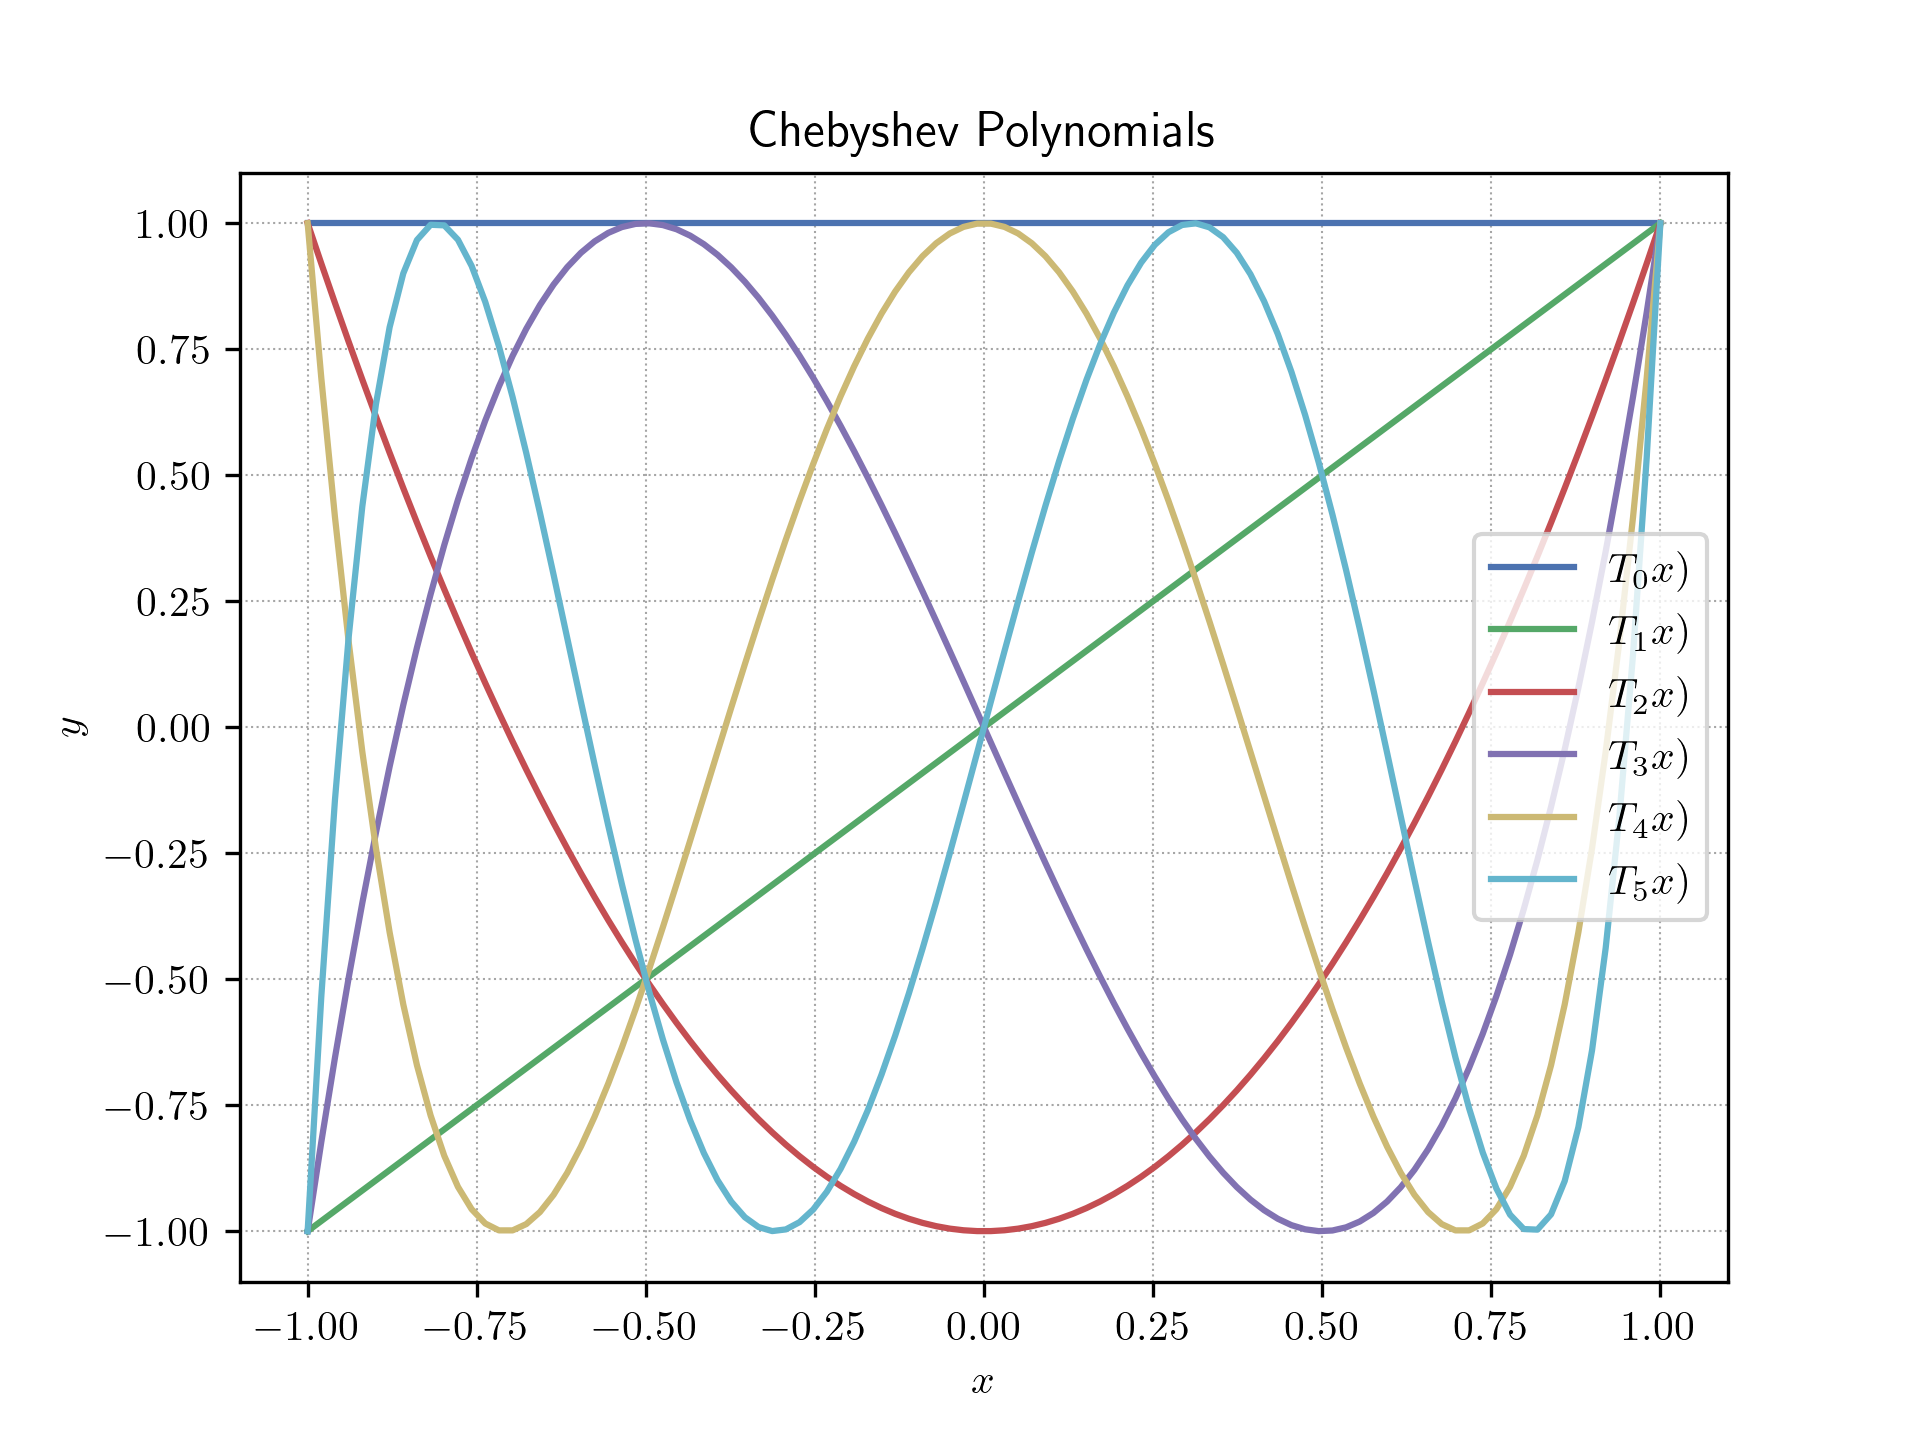
\includegraphics[width=0.8\textwidth]{../plots_2/q3_4/chebyshev_polys.png}
\end{center}

\newpage
\question{Lagrange Interpolation for Nonsmooth Function}
Let $f(x) = |x|$ on the interval $[-1,1]$.

\subquestion
Construct the interpolation polynomial $P_n(x)$ for equidistant nodes when $n$ is even.

\solution The interpolation polynomial $P_n(x)$ can be constructed using the Lagrange interpolation formula:
\[
P_n(x) = \sum_{i=0}^{n} f(x_i) \prod_{\substack{0 \leq j \leq n \\ j \neq i}} \frac{x - x_j}{x_i - x_j}
\]
where $x_i$ are the equidistant nodes in the interval $[-1, 1]$. For even $n$, the nodes are given by:
\[
x_i = -1 + \frac{2i}{n}, \quad i = 0, 1, \ldots, n
\]
Substituting $f(x) = |x|$ into the Lagrange formula gives that:
\[P_n(x) = \sum_{i=0}^{n} |x_i| \prod_{\substack{0 \leq j \leq n \\ j \neq i}} \frac{x - x_j}{x_i - x_j}\]

\subquestion
Show that $P_n(x)$ is an even polynomial.

\begin{proof}
    To show that $P_n(x)$ is an even polynomial, we need to show that $P_n(-x) = P_n(x)$ for all $x$ in the interval $[-1, 1]$.

    From the previous part, we have that:
    \[P_n(x) = \sum_{i=0}^{n} |x_i| L_i(x)\]
    where
    \[L_i(x) = \prod_{\substack{0 \leq j \leq n \\ j \neq i}} \frac{x - x_j}{x_i - x_j}\]
    is the Lagrange basis polynomial. If we plug in $-x$ into $P_n(x)$, we have:
    \[P_n(-x) = \sum_{i=0}^{n} |x_i| L_i(-x)\]
    Let us first focus on $L_i(-x)$.
    Since $n$ is even, we have that the nodes $x_i$ are symmetric about $0$. So we have that for each node $x_i$, there exists a corresponding node $x_{n-i} = -x_i$. Starting with $L_i(-x)$, we have:
    \[L_i(-x) = \prod_{\substack{0 \leq j \leq n \\ j \neq i}} \frac{-x - x_j}{x_i - x_j}\]
    Let focus on each factor in the product and let $x_i = -x_{n-i}$, $x_j = -x_{n-j}$. Then, we have:
    \[\frac{-x - x_j}{x_i - x_j} = \frac{-x + x_{n-j}}{-x_{n-i} + x_{n-j}} = \frac{-(x - x_{n-j})}{-(x_{n-i} - x_{n-j})} = \frac{x - x_{n-j}}{x_{n-i} - x_{n-j}}\]
    Therefore, we can rewrite $L_i(-x)$ as:
    \[L_i(-x) = \prod_{\substack{0 \leq j \leq n \\ j \neq i}} \frac{x - x_{n-j}}{x_{n-i} - x_{n-j}}\]
    Note that as $j$ goes from $0$ to $n$, $j \neq i$, $n-j$ goes from $n$ to $0$ and $n-j \neq n-i$, and $n-i$ goes from $n$ to $0$. This is just the original product in backwards order. Letting $m = n-j$, we can rewrite the product as:
    \[L_i(-x) = \prod_{\substack{0 \leq m \leq n \\ m \neq n-i}} \frac{x - x_{m}}{x_{n-i} - x_{m}} = L_{n-i}(x) \label{L}\tag{1}\]
    Now reconsidering $P_n(-x)$, we have:
    \[P_n(-x) = \sum_{i=0}^{n} |x_i| L_i(-x)\]
    Using \eqref{L}, we can rewrite this as:
    \[P_n(-x) = \sum_{i=0}^{n} |x_i| L_{n-i}(x)\]
    By the symmetry of the nodes, we have that $|x_i| = |-x_{n-i}| = |x_{n-i}|$. So:
    \[P_n(-x) = \sum_{i=0}^{n} |x_{n-i}| L_{n-i}(x)\]
    Letting $m = n-i$, we can rewrite the sum as:
    \[P_n(-x) = \sum_{m=0}^{n} |x_{m}| L_{m}(x) = P_n(x)\]
    Therefore have shown that $P_n(-x) = P_n(x)$ for all $x$ in the interval $[-1, 1]$. So $P_n(x)$ is an even polynomial.
\end{proof}

\newpage

\subquestion
Investigate analytically (for small $n$) how well $P_n(x)$ approximates $f(x)$.

\solution The remainder term for Lagrange interpolation is given by:
\[R_n(x) = f(x) - P_n(x) = |x| - P_n(x), \quad x \in [-1, 1]\]
Since $f(x)$ and $P_n(x)$ are both even functions, $R_n(x)$ is also an even function. Therefore, we only need to analyze $R_n(x)$ on the interval $[0, 1]$. Let us analyze $\max_{x \in [0,1]} |R_n(x)|$ for small even $n=2k$.
Note that we may rewrite $R_n(x)$ as:
\[R_n(x) = x - P_n(x), \quad x \in [0, 1]\]

Since $P_n(x)$ is even, all odd constants ($a_{2k-1}, a_{2k-3}, \ldots, a_1$) must vanish. Also, given that $n=2k$ is even, we have that $0$ is always a node. Therefore, we have that $P_n(0) = a_{2k}x^{2k} + a_{2k-2}x^{2k-2} + \dots + a_2x^2 + a_0 = f(0) = 0$. So $a_0 = 0$.

\textbf{Case: $n=2$}

Our nodes are $\{-1, 0, 1\}$.

Note $P_2(x)$ must be of the form: 
\[P_2(x) = a_2x^2\]
So we have:
\[P_2(1) = a_2 = 1\] 
Therefore, we have:
\[P_2(x) = x^2\]
So the remainder term is:
\[R_2(x) = x - x^2, \quad x \in [0, 1]\]
To find the maximum error, we can take the derivative of $R_2(x)$ and set it to $0$:
\[R_2'(x) = 1 - 2x = 0\]
\[\implies x = \frac{1}{2}\]
Evaluating $|R_2(x)|$ at the critical point (note: maximum cannot occur at endpoint by construction):
\[|R_2\left(\frac{1}{2}\right)| = \frac{1}{2} - \frac{1}{4} = \frac{1}{4}\]
So the maximum error occurs at $x = \frac{1}{2}$ and is:
\[\max_{x \in [0,1]} |R_2(x)| =\frac{1}{4} = 0.25\] 

\textbf{Case: $n=4$}

Our nodes are $\{-1, -\frac{1}{2}, 0, \frac{1}{2}, 1\}$.

Note $P_4(x)$ must be of the form:
\[P_4(x) = a_4x^4 + a_2x^2\]
So we have the following system of equations:
\[P_4(1) = a_4 + a_2 = 1\]
\[P_4\left(\frac{1}{2}\right) = \frac{a_4}{16} + \frac{a_2}{4} = \frac{1}{2}\]
Rewriting the second equation, we have:
\[a_4 + 4a_2 = 8\]
Solving this system of equations, we get:
\[a_4 = -\frac{4}{3}, \quad a_2 = \frac{7}{3}\]
So therefore:
\[P_4(x) = -\frac{4}{3}x^4 + \frac{7}{3}x^2\]
As a result, our remainder term is:
\[R_4(x) = x - \left(-\frac{4}{3}x^4 + \frac{7}{3}x^2\right) = x + \frac{4}{3}x^4 - \frac{7}{3}x^2, \quad x \in [0, 1]\]
Again, to find the maximum error, we can take the derivative of $R_4(x)$ and set it to $0$:
\[R_4'(x) = 1 + \frac{16}{3}x^3 - \frac{14}{3}x = 0\]
We may use the cubic formula to find the roots of this equation. Using \href{https://www.wolframalpha.com/widgets/view.jsp?id=3f4366aeb9c157cf9a30c90693eafc55}{WolframAlpha}, we find that the roots in the interval $[0,1]$ are approximately $x \approx 0.22779, 0.80048$. By the Runge phenomenon, we expect the maximum error to occur in the last sub-interval $[\frac{1}{2}, 1]$. Evaluating $|R_4(x)|$ at the critical points of the interval, we have:
\[|R_4(0.22779)| \approx 0.1103071958\]
\[|R_4(0.80048)| \approx 0.1472006375\]
So the maximum error occurs at $x \approx 0.80048$ and is approximately:
\[\max_{x \in [0,1]} |R_4(x)| \approx 0.1472006375\]

For higher even $n$, a similar approach can be used to find $P_n(x)$ and analyze the error. The roots of $R_n'(x)$ can be found using numerical methods such as Newton's method or the bisection method since they don't have closed-form solutions.

To avoid the heavy computation, we can observe $|R_n(x)|$ graphically for different $n$. A modified version of the code from question 2.2 was used to plot $f(x)$, $P_n(x)$, and $|R_n(x)|$ for even $n=2, 4, 6, 8$ (see Appendix).

\newpage

The following plots show $f(x)$ and $P_n(x)$ for even $n=2, 4, 6, 8$:
\begin{center}
    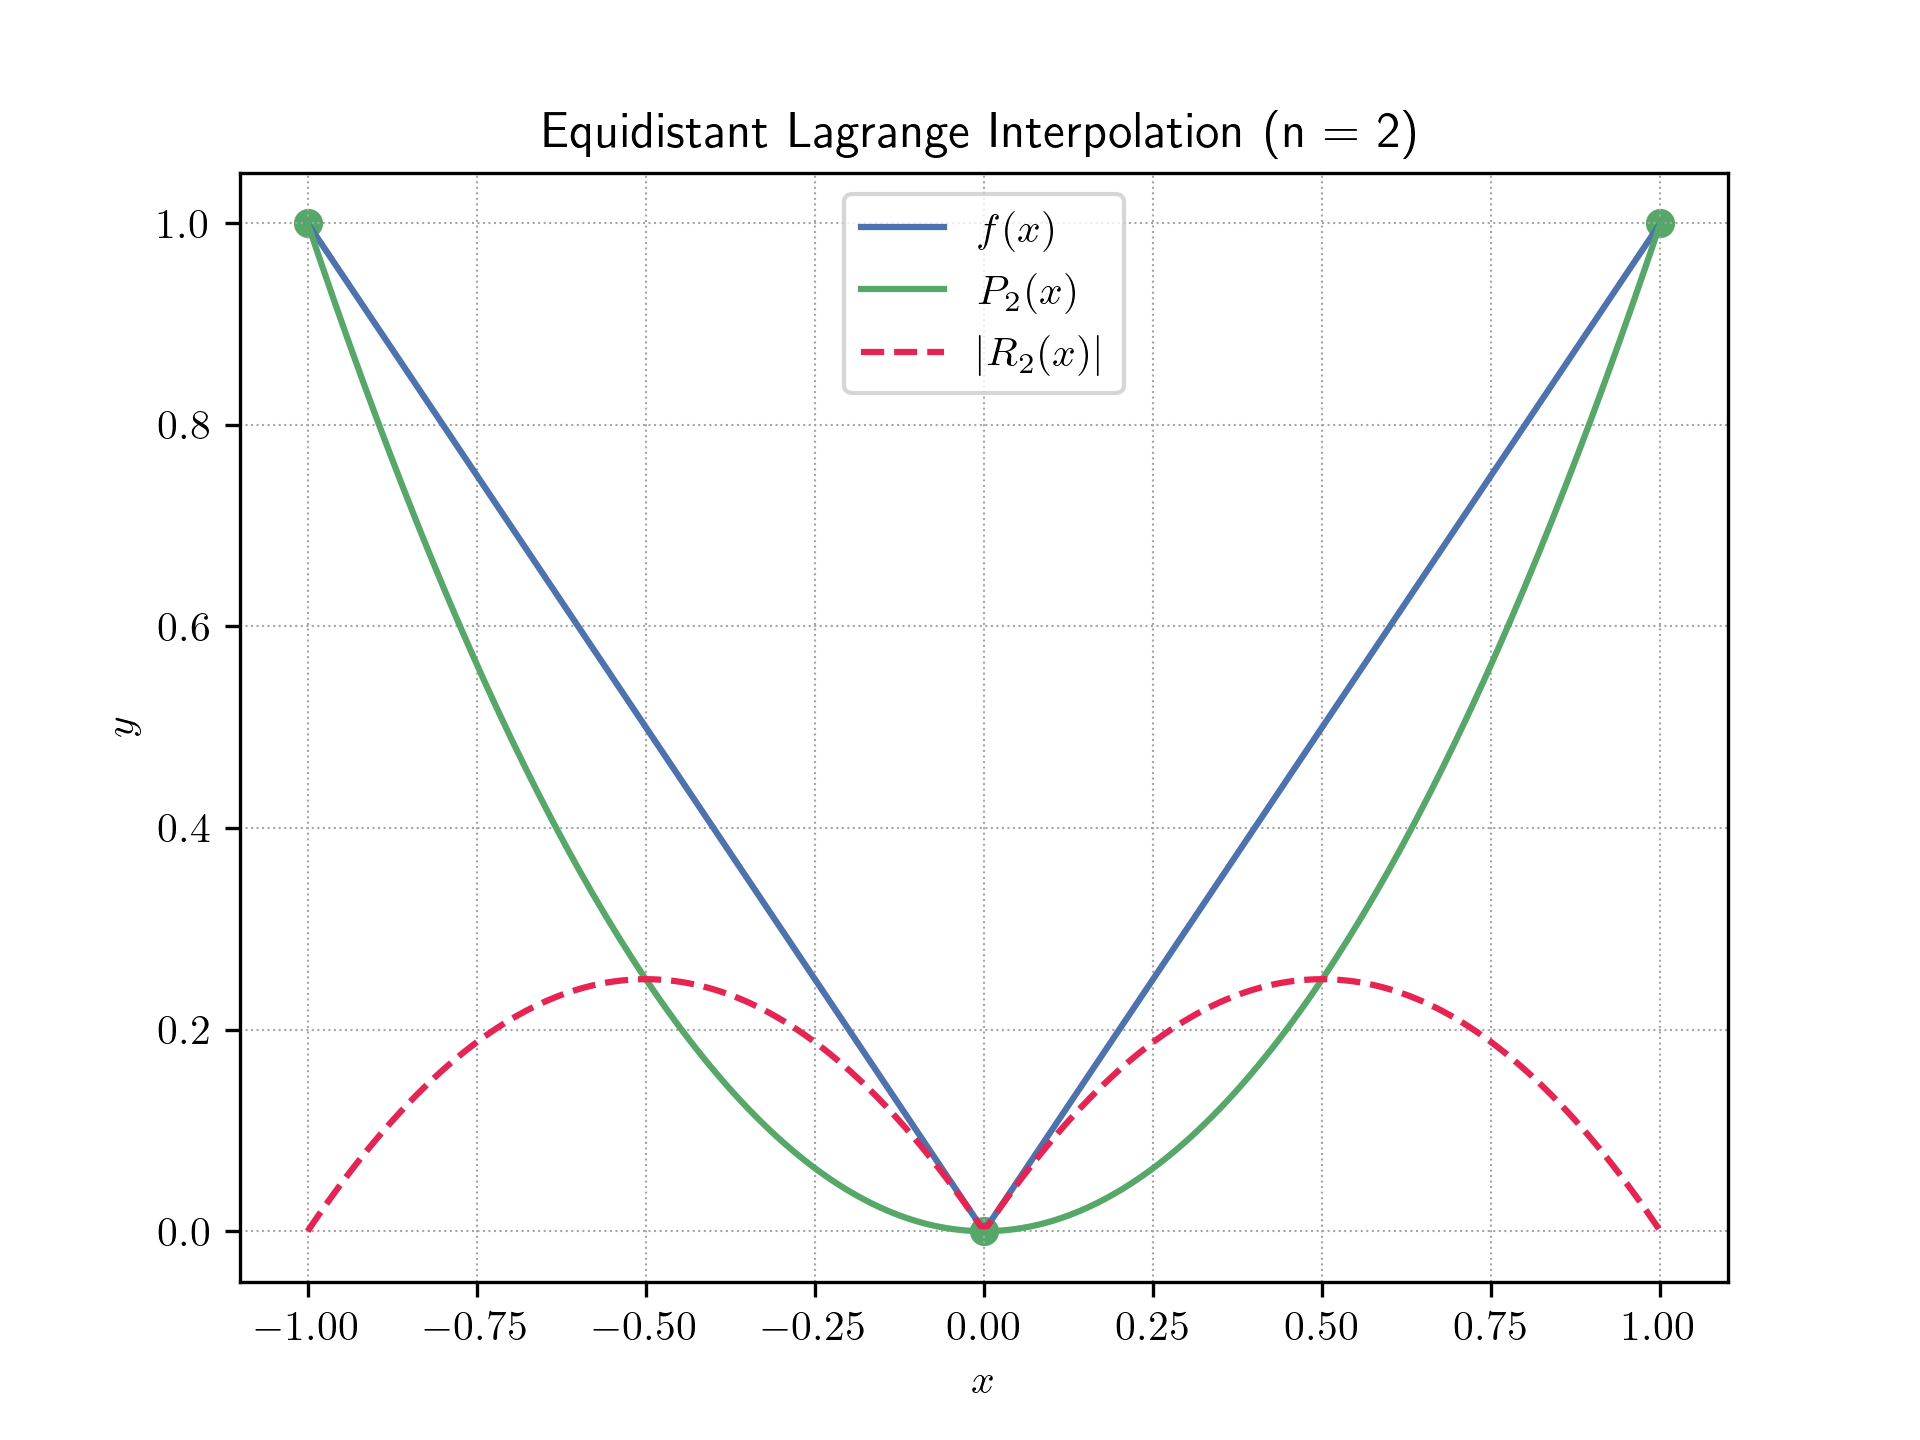
\includegraphics[width=0.8\textwidth]{../plots_2/q4_3/p2.png}
    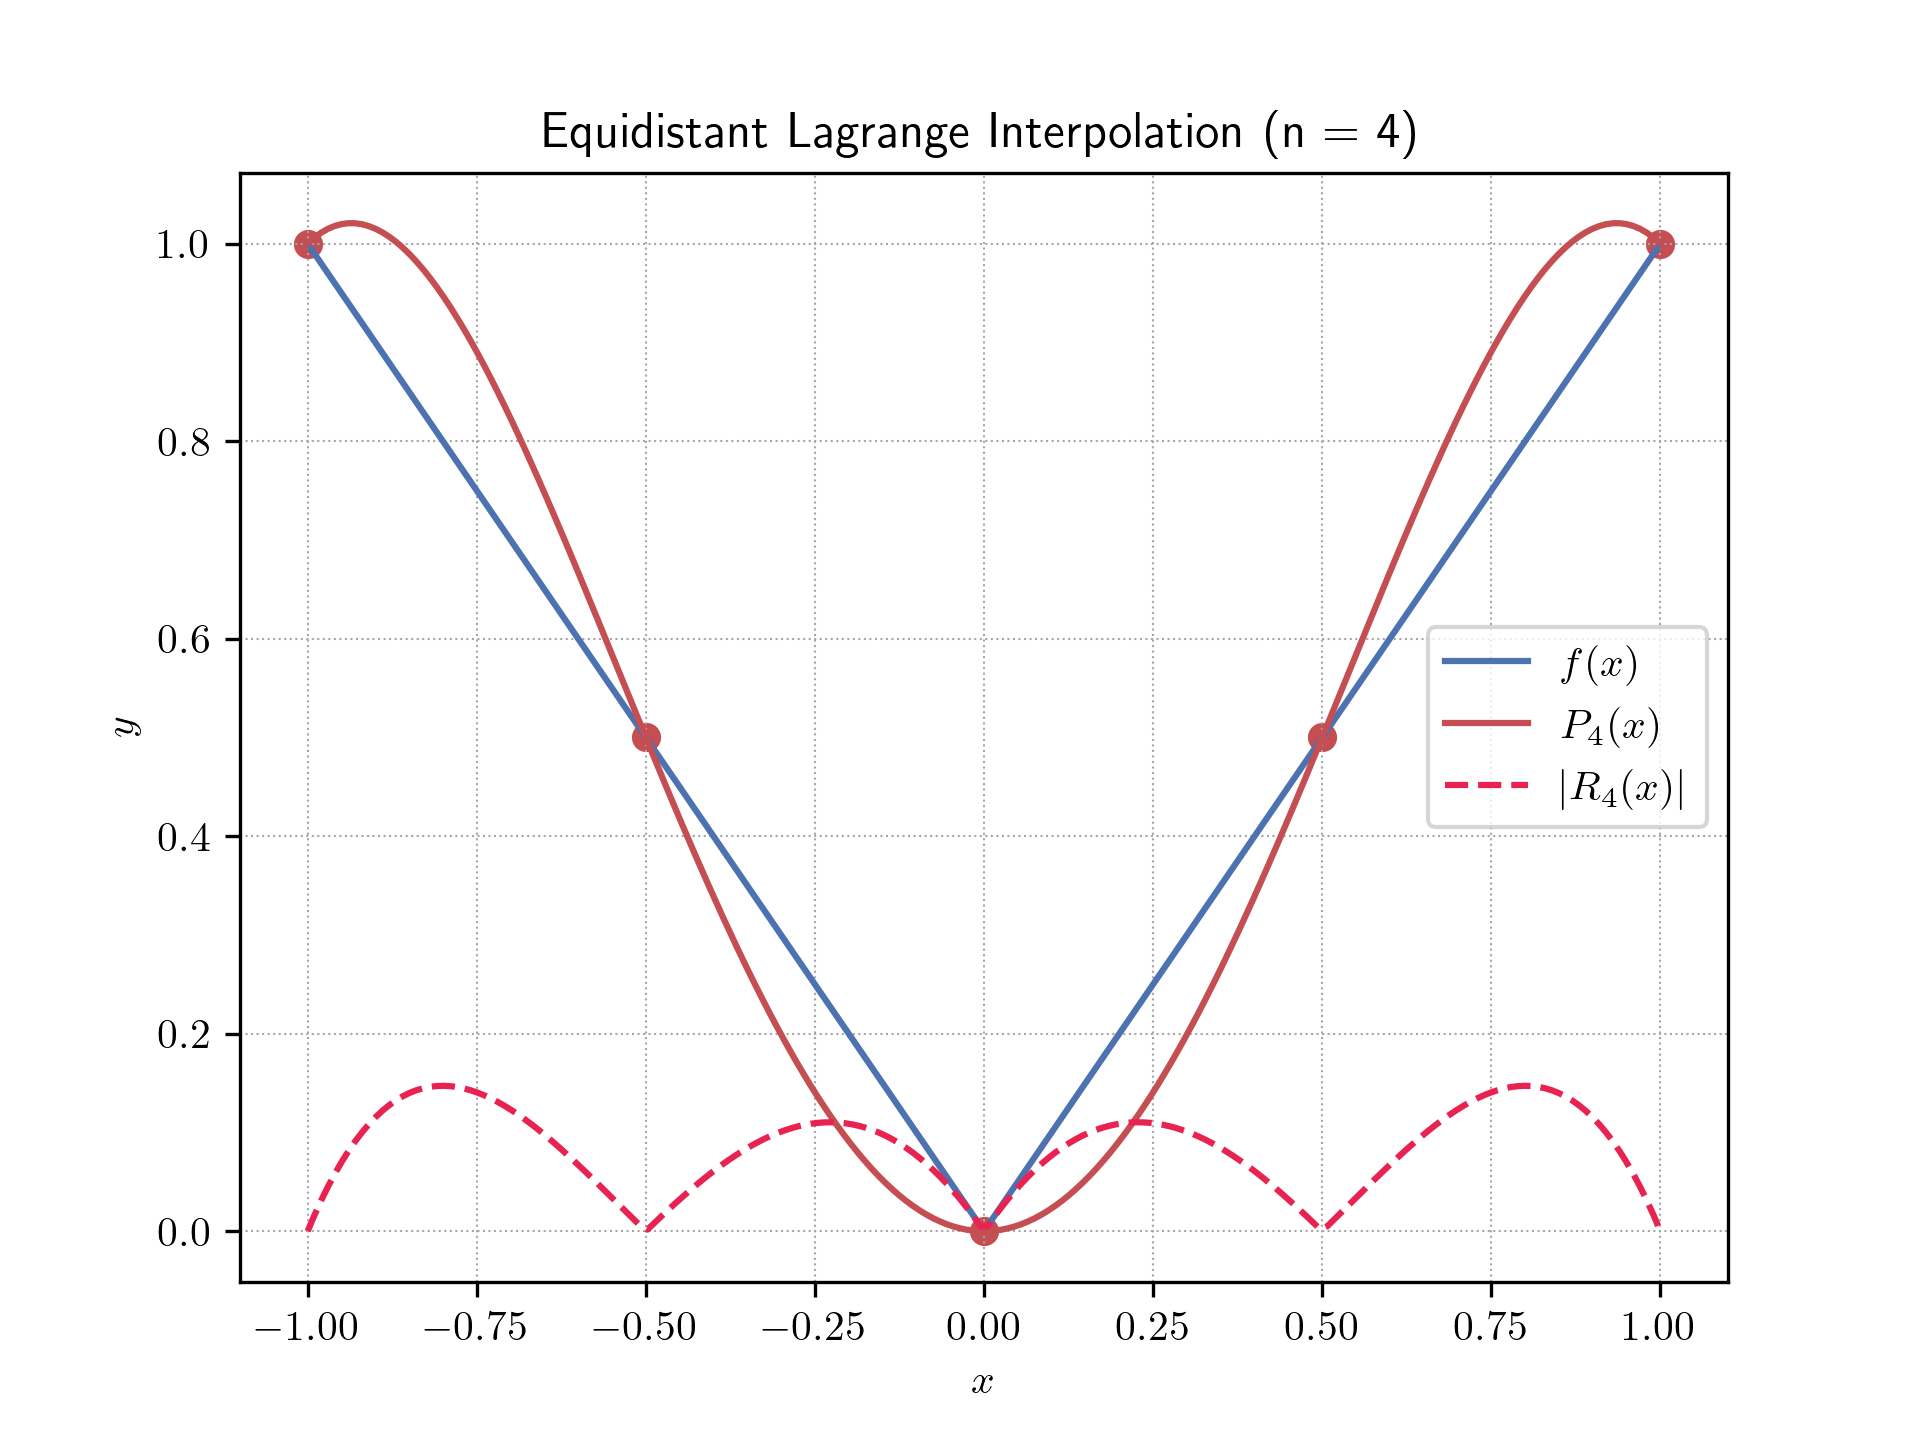
\includegraphics[width=0.8\textwidth]{../plots_2/q4_3/p4.png}
    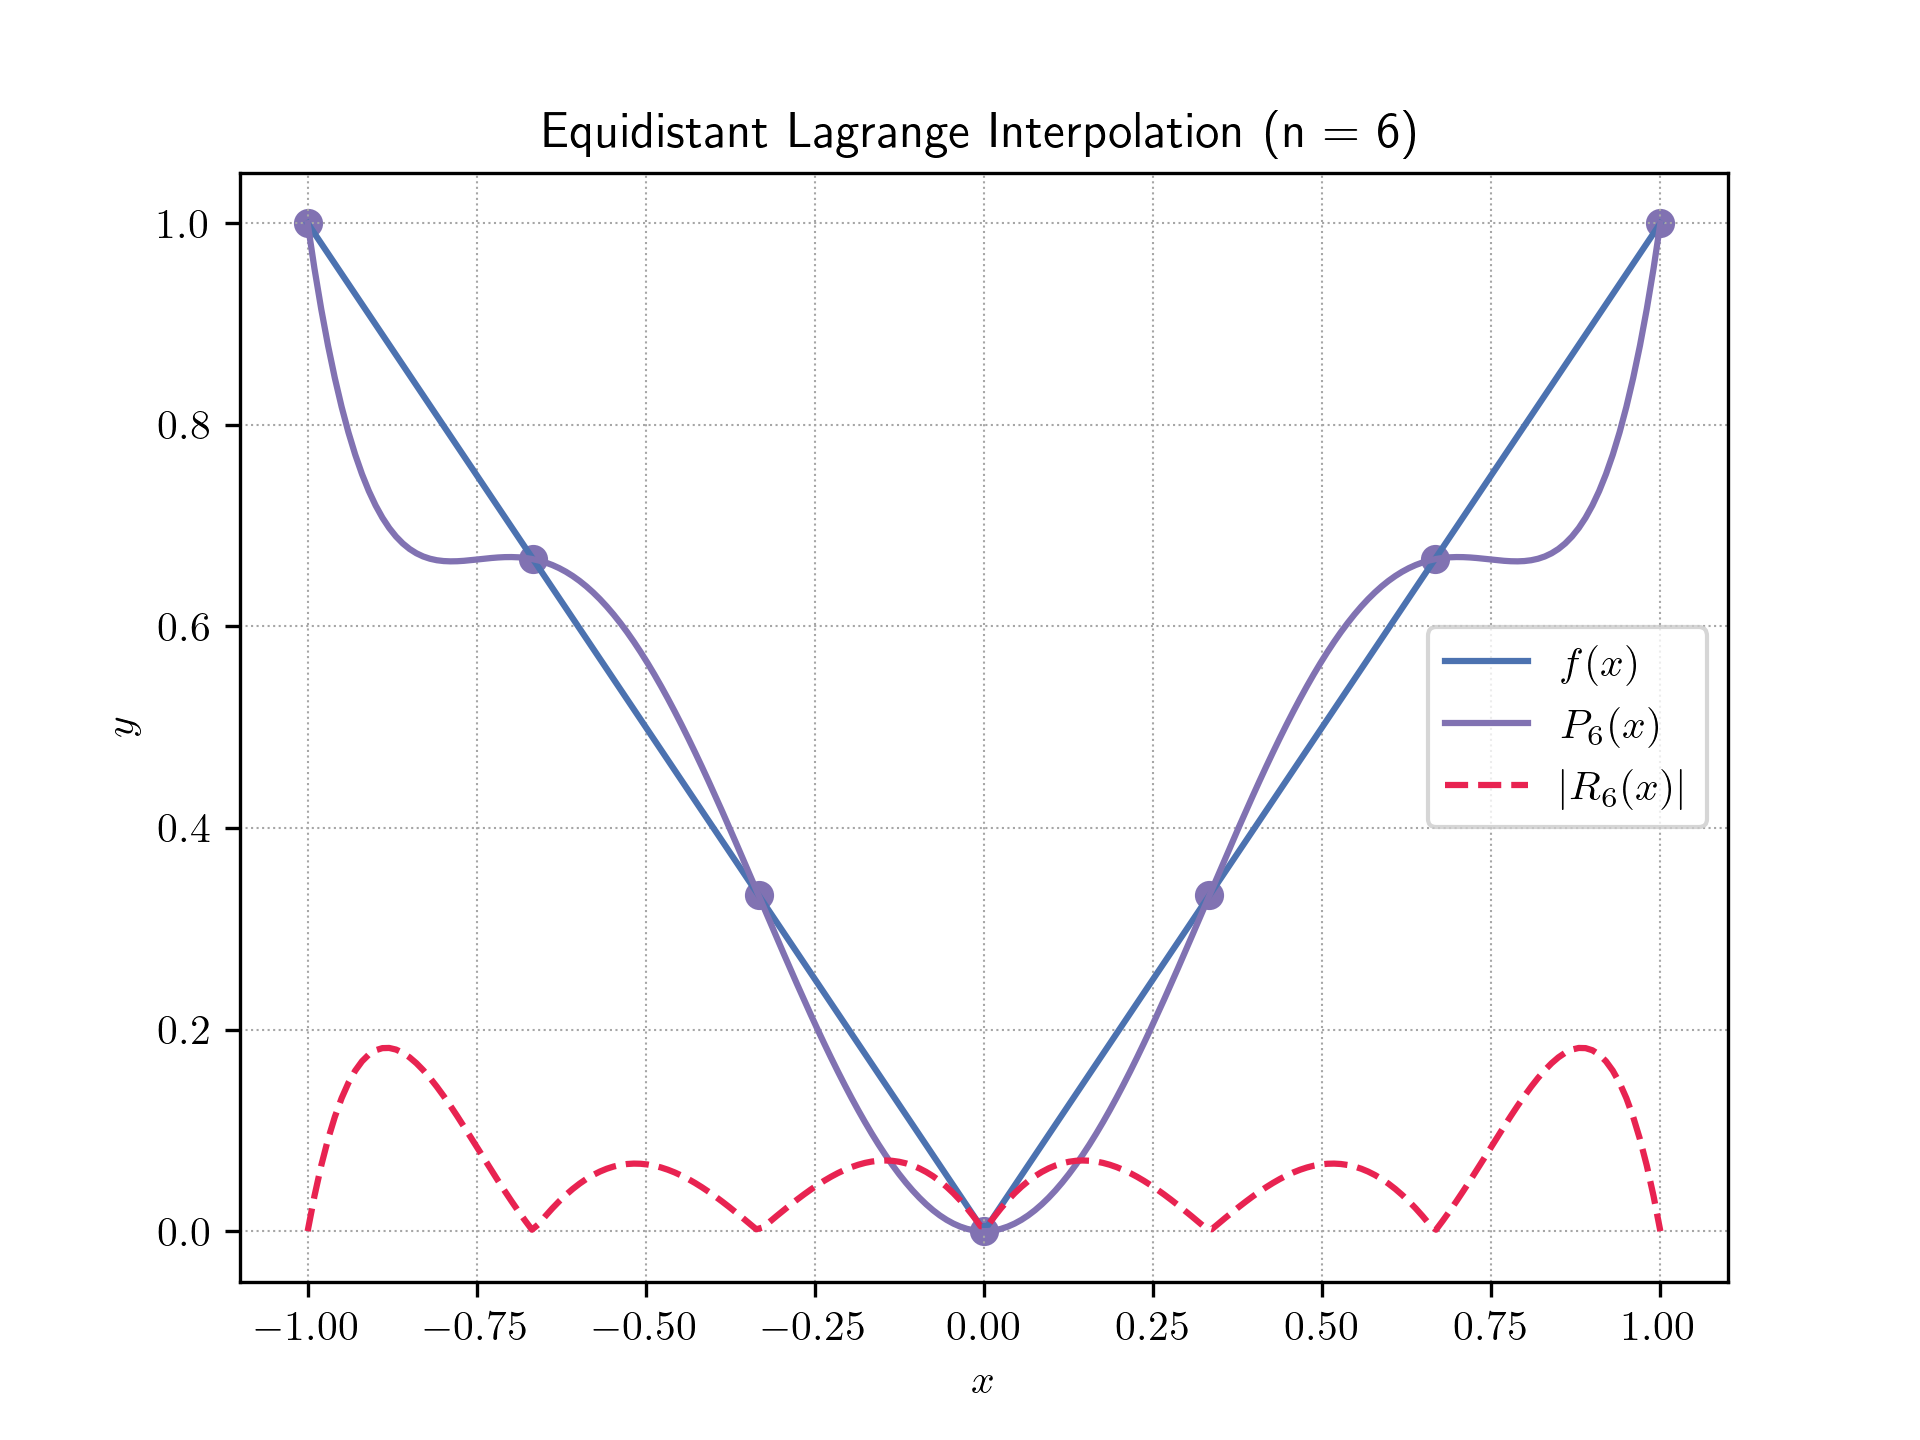
\includegraphics[width=0.8\textwidth]{../plots_2/q4_3/p6.png}
    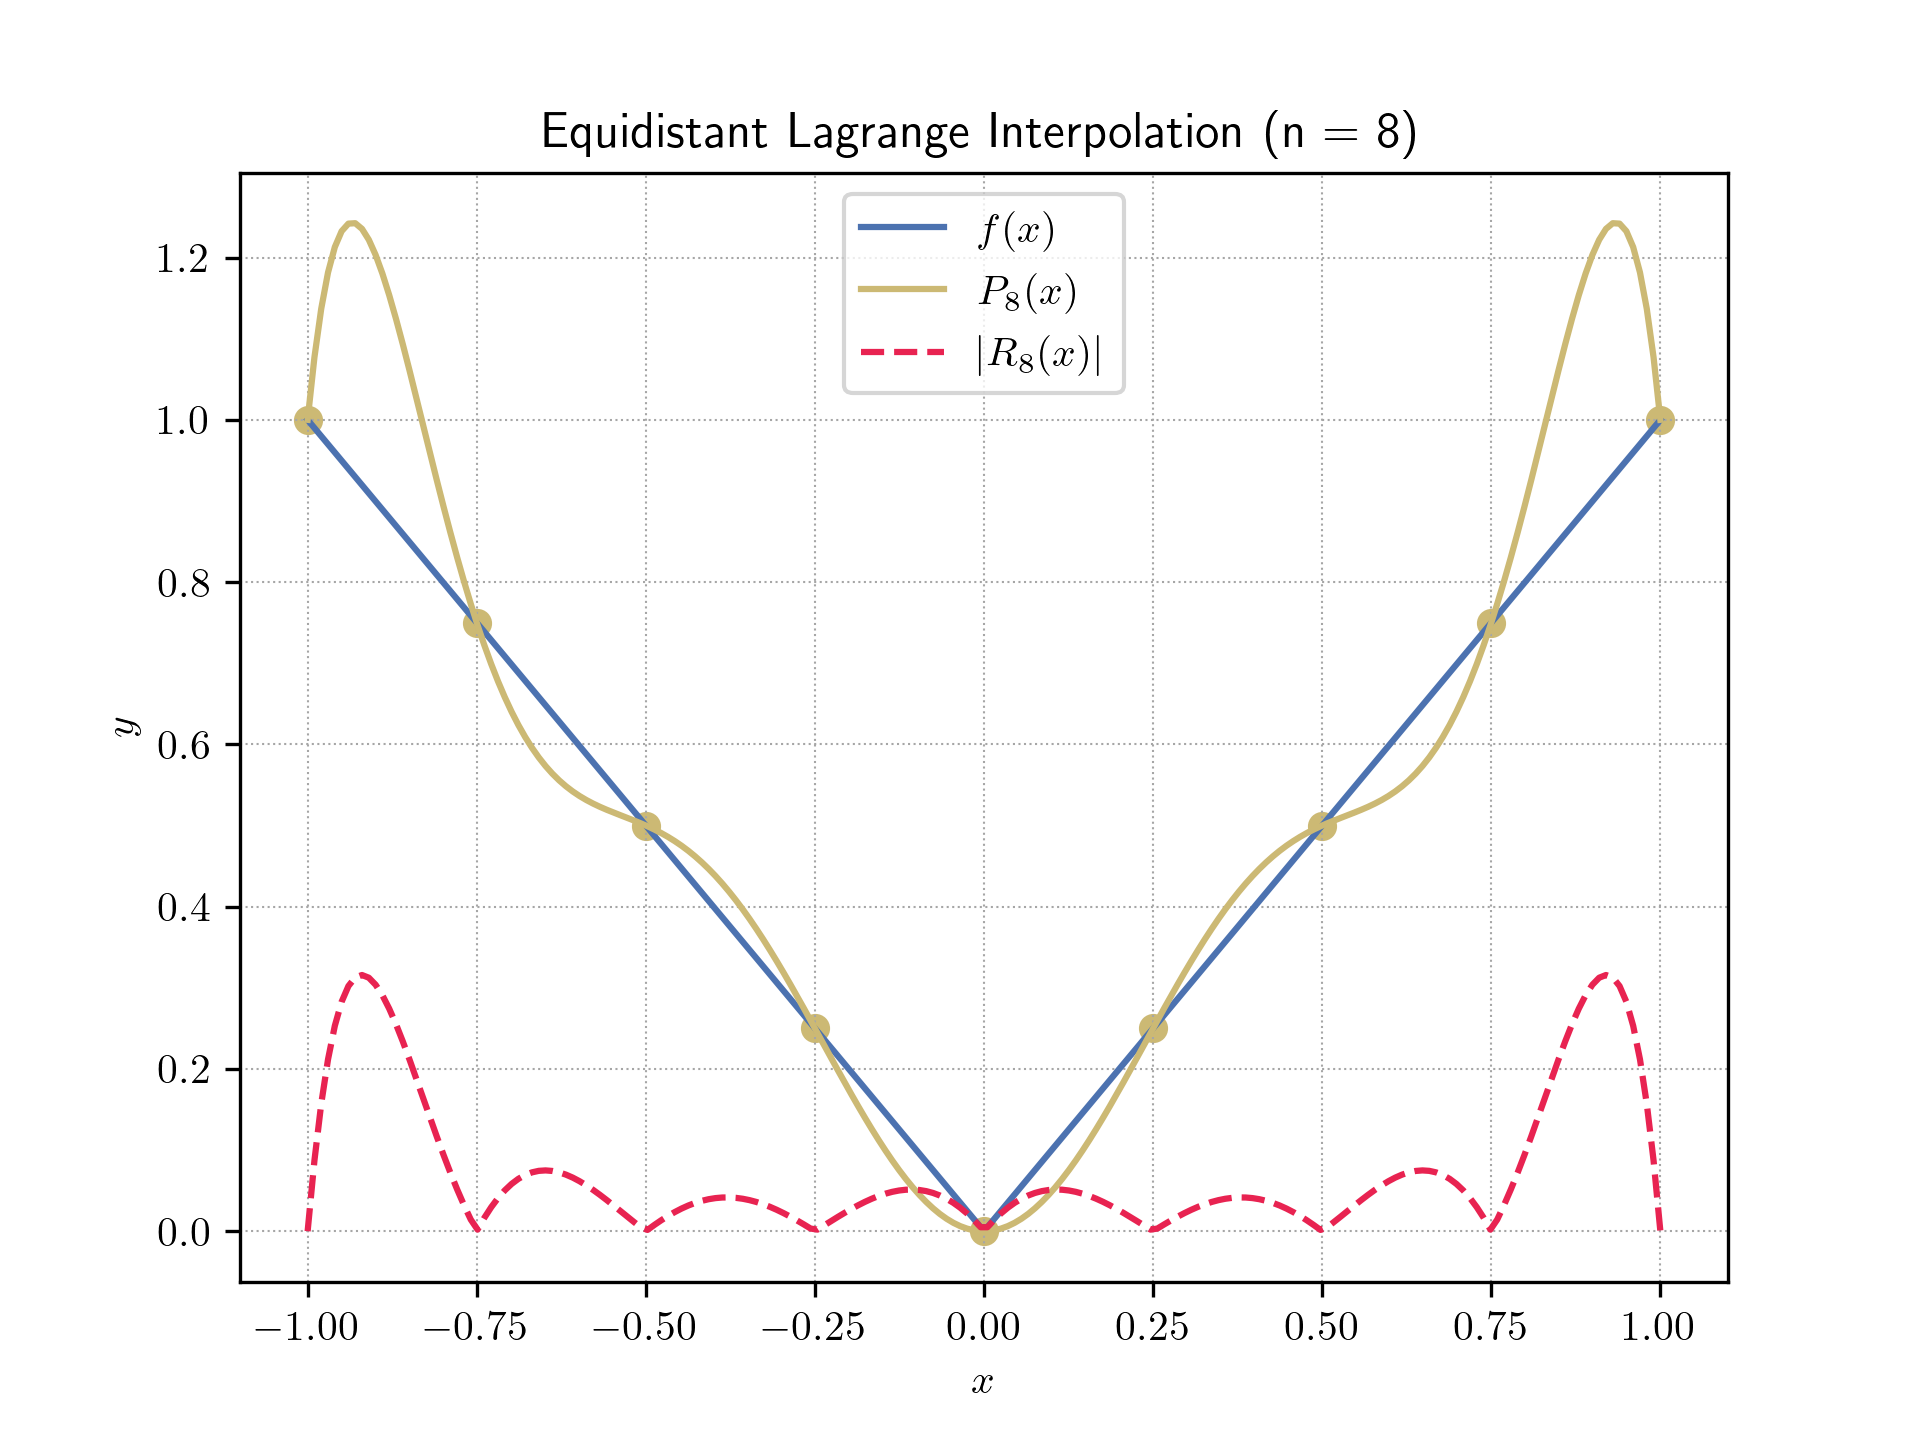
\includegraphics[width=0.8\textwidth]{../plots_2/q4_3/p8.png}
    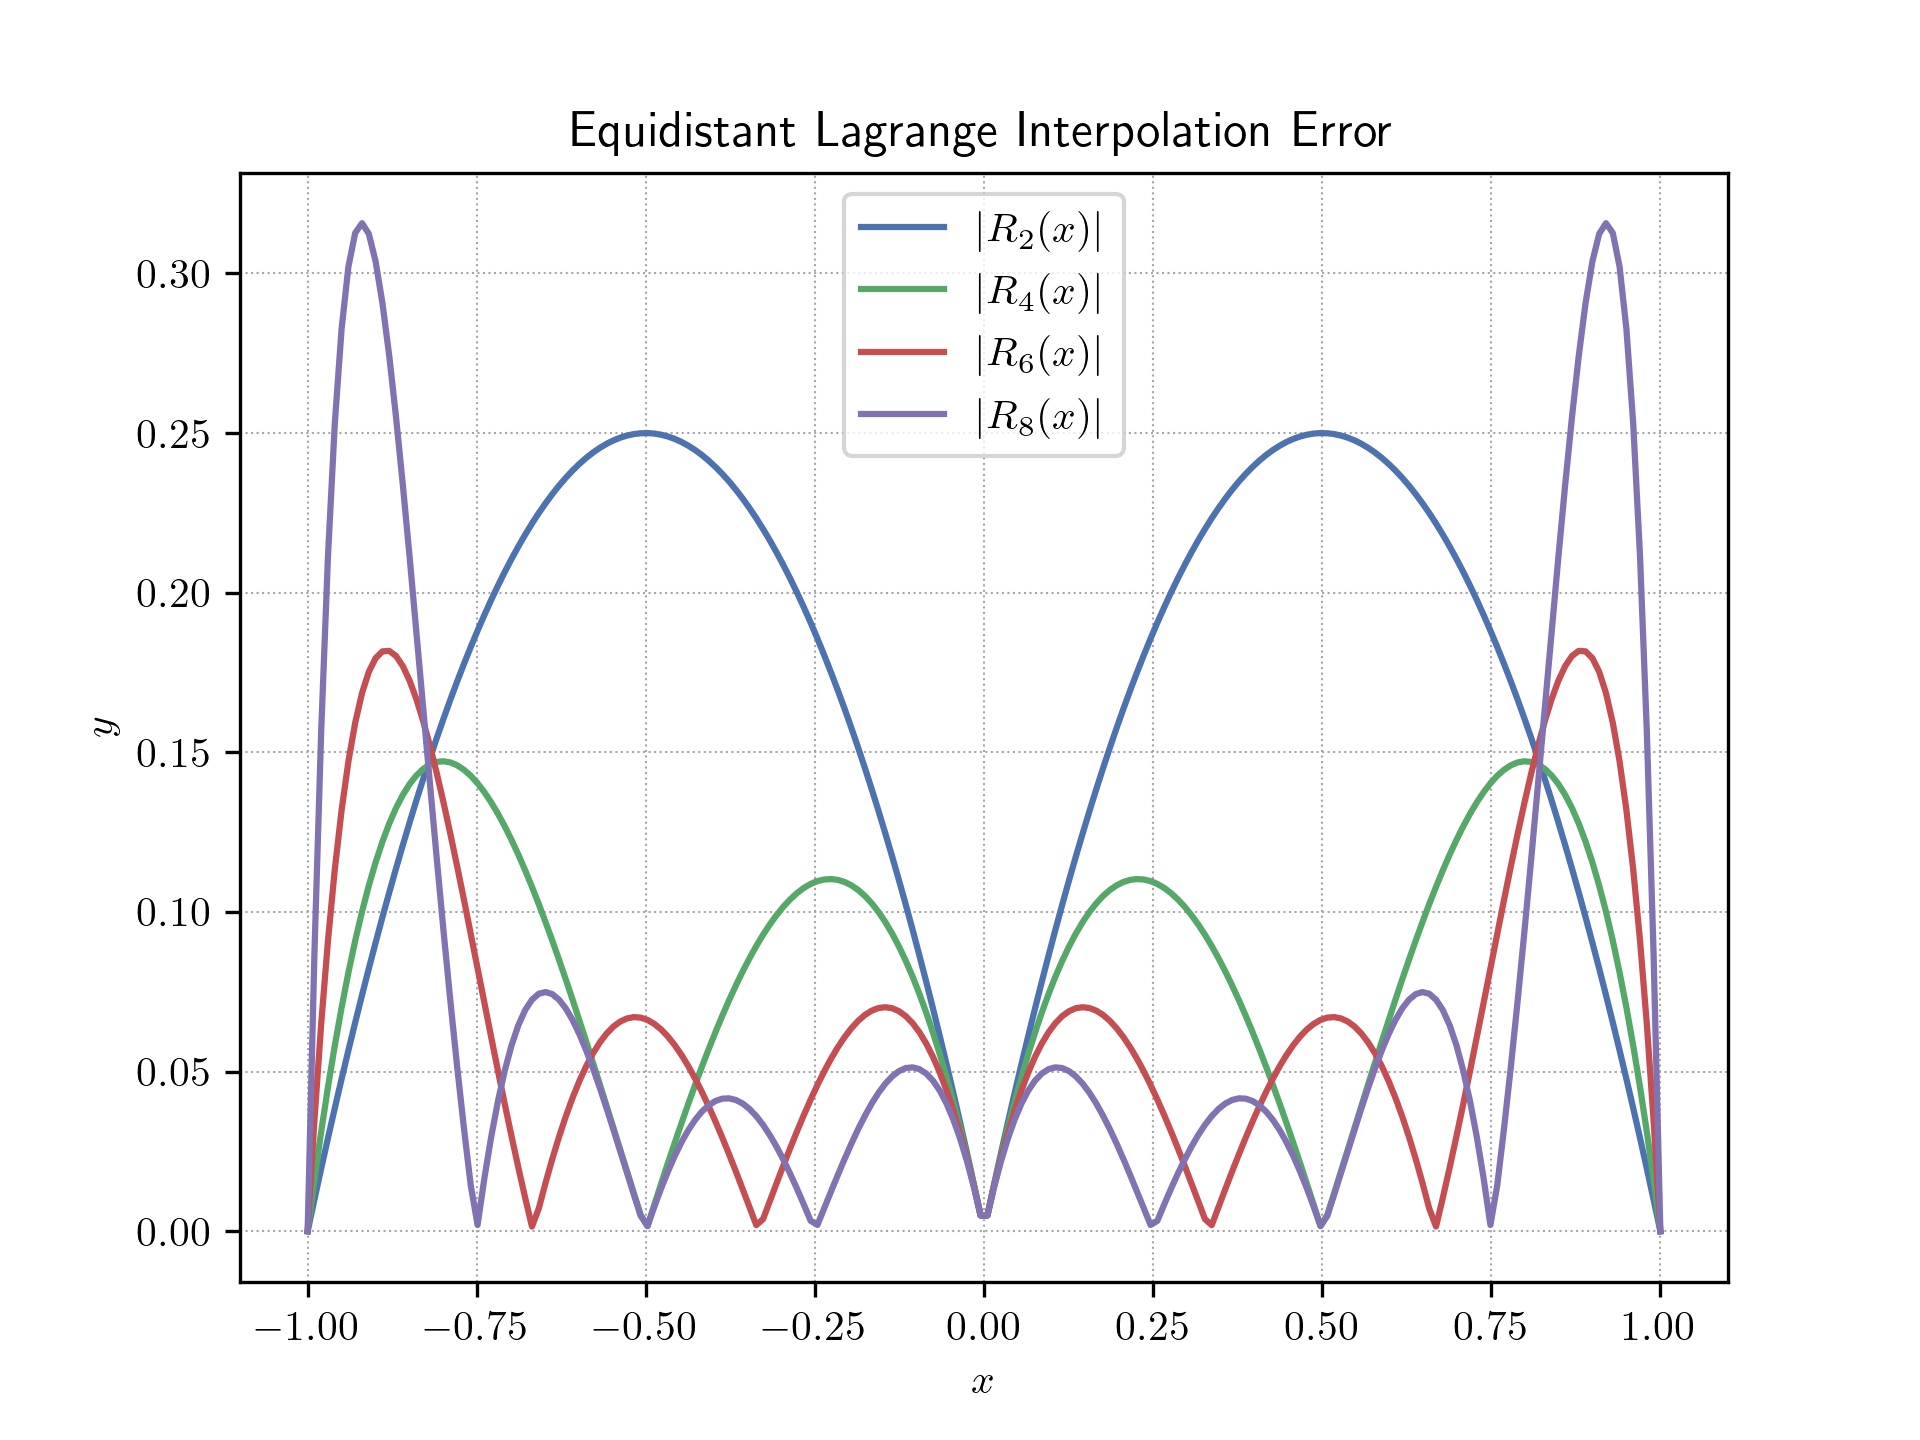
\includegraphics[width=0.8\textwidth]{../plots_2/q4_3/error.png}
\end{center}

We note that initially, $\max_{x \in [0,1]} |R_n(x)|$ decreases from $n=2$ (0.25) to $n=4$ (0.1472006375). However, starting from $n=6$, the maximum error (roughly 0.18) starts to increase again occurring near the endpoints. This trend continues, eventually surpassing the maximal error for $n=2$ (0.25) at $n=8$ (roughly 0.315). Since our nodes are equally spaced, this is an observation of the Runge phenomenon. Centrally, the error decreases as $n$ increases, but near the endpoints, the error increases significantly.

\newpage

\subquestion
Discuss why convergence may be slower for nonsmooth functions.

\solution
Nonsmooth functions, such as $f(x) = |x|$, have points where they are not differentiable. In the case of $f(x) = |x|$, $f$ is not differentiable at $x=0$. This lack of smoothness can lead to larger interpolation errors, especially near the nonsmooth points. Since our n is even, we always have a node at $x=0$. However, if $n$ were odd, we would not have a node at $0$, and the interpolation error would nonzero at this point. Since Lagrange interpolation uses smooth basis polynomials to approximate $f$, it may not be able to accurately capture the behavior of the nonsmooth function near these points, leading to slower convergence.

This effect is more apparent when interpolating functions that are near vertical or have jump discontinuities. When using Fourier series to approximate such functions (like a step function), we can observe the Gibbs phenomenon, where oscillations occur near the discontinuities. These oscillations do not diminish as more terms are added to the series, leading to a persistent error near the discontinuity. Similarly, for polynomial interpolation of nonsmooth functions, we may observe oscillatory behavior near the nonsmooth points, leading to slower convergence.

\newpage
{\Large\textbf{Appendix}}

This appendix contains the complete code used for Assignment 2.

\lstinputlisting[language=Python, caption={assignment\_2.py}]{../assignment_2.py}

\end{document}